\documentclass[11pt]{manual} %manual
\usepackage[utf8]{inputenc}
\usepackage{geometry}                % See geometry.pdf to learn the layout options. There are lots.
\geometry{a4paper}                   % ... or a4paper or a5paper or ... 
%\geometry{landscape}                % Activate for for rotated page geometry
%\usepackage[parfill]{parskip}    % Activate to begin paragraphs with an empty line rather than an indent
\usepackage{graphicx}
\usepackage{listings}
\usepackage{color}
%\usepackage{amssymb}
\usepackage{makeidx}
\usepackage{url}
\usepackage{colortbl}
\usepackage[table]{xcolor}
\definecolor{seagreen}{RGB}{87,135,159}
\definecolor{light-gray}{gray}{0.85}
\definecolor{medium-gray}{gray}{0.5}
\usepackage[colorlinks=true,linkcolor= seagreen]{hyperref}

% add counter to paragraphs and change counter to Roman for the chapter
\setcounter{secnumdepth}{4}
\renewcommand{\thechapter}{\Roman{chapter}}
\makeatletter
\renewcommand\paragraph{\@startsection{paragraph}{4}{\z@}%
{3.25ex \@plus1ex \@minus.2ex}%
{1.5ex \@plus.2ex}%
{\normalfont\normalsize\bfseries}}
\renewcommand\subparagraph{\@startsection{subparagraph}{5}{\z@}%
{3.25ex \@plus1ex \@minus.2ex}%
{1.5ex \@plus.2ex}%
{\normalfont\normalsize\bfseries\underline}}
\makeatother

\title{Trampoline on targets}
\author{Florent PAVIN}
%% LSTLISTING %%
\lstset{ %
language=sh,                % choose the language of the code
basicstyle=\small,       % the size of the fonts that are used for the code
%numbers=left,                   % where to put the line-numbers
%numberstyle=\footnotesize,      % the size of the fonts that are used for the line-numbers
%stepnumber=2,                   % the step between two line-numbers. If it's 1 each line will be numbered
%numbersep=5pt,                  % how far the line-numbers are from the code
backgroundcolor=\color{white},  % choose the background color. You must add \usepackage{color}
showspaces=false,               % show spaces adding particular underscores
showstringspaces=false,         % underline spaces within strings
showtabs=false,                 % show tabs within strings adding particular underscores
tabsize=2,			% sets default tabsize to 2 spaces
captionpos=b,			% sets the caption-position to bottom
breaklines=true,		% sets automatic line breaking
breakatwhitespace=false,	% sets if automatic breaks should only happen at whitespace
escapeinside={\%*}{*)},          % if you want to add a comment within your code
columns=flexible,
commentstyle=\color{blue},
morekeywords={rm,dirname,set,bunzip2,tar,mkdir,time,mv,sudo},keywordstyle=\color{black}\bfseries,
morecomment=[s][\color{red}]{"}{"},
frame=leftline|topline|bottomline|rightline
}

%\lstset{
%  language=goilTemplate,
%  emph={
%    var,
%    expression,
%    string,
%    instruction_list,
%    template_file_name,
%    reader,
%    hierarchy
%  },
%  emphstyle=\em,
%  moredelim=[s][\color{blue}]{\%}{\%},
%  moredelim=[s]{"}{"},
%  morecomment=[l][\color{medium-gray}\itshape]{\#},
%  basicstyle=\ttfamily\small
%}

\release{1.0}
\makeindex

\begin{document}
\maketitle
~\newpage
\setcounter{tocdepth}{3}
\tableofcontents

\chapter{Getting started on an example}

%%%%%%%%%%%%%%%%%
This document describes how to get started a Trampoline \footnote{Trampoline is an open source RTOS which, once certified, could be compliant with the OSEK/VDX specification. Currently it is not the case, so while Trampoline has the same API as OSEK/VDX, it is not officially compliant. Trampoline is available under the GNU Lesser General Public License V2 and \textbf{is maintained by gcc-4.0.1}. Trampoline runs on several platforms like POSIX, C166 with Keil compiler, Star12X (courtesy of Geensys), PowerPC, ARM (NXT2 for example)} application on any target.\\
The following steps will be overviewed :
\begin{itemize}
\item Trampoline installation
\item Target Compiler needed
\item Installation of drivers and softwares to be able to upload programs on your board.
\end{itemize}
This document is explained from a UNIX side. If you are on a Windows system, download and install Cygwin as it is explained on NXTOSEK website (\href{http://lejos-osek.sourceforge.net/installation_windows.htm}{http://lejos-osek.sourceforge.net/installation\_windows.htm}) first.

\documentclass[11pt]{manual}
\usepackage[utf8]{inputenc}
\usepackage[footnotesep=15pt,foot=40pt]{geometry}                % See geometry.pdf to learn the layout options. There are lots.
\geometry{a4paper}                   % ... or a4paper or a5paper or ... 
%\geometry{landscape}                % Activate for for rotated page geometry
%\usepackage[parfill]{parskip}    % Activate to begin paragraphs with an empty line rather than an indent
\usepackage{graphicx}
\usepackage{listings}
\usepackage{color}
%\usepackage{amssymb}
\usepackage{makeidx}
\usepackage{url}
\usepackage{colortbl}
\usepackage[table]{xcolor}
\usepackage{longtable}
\usepackage{underscore}
\usepackage{caption}

\renewcommand{\captionlabelfont}{\small \bf}
\renewcommand{\captionfont}{\small \it}

\definecolor{seagreen}{RGB}{64,100,120}
\definecolor{darkpink}{RGB}{200,100,120}
\definecolor{light-gray}{gray}{0.85}
\definecolor{medium-gray}{gray}{0.5}
\usepackage[colorlinks=true,linkcolor=seagreen,citecolor=darkpink]{hyperref}
\usepackage{supertabular} %supertabular

\usepackage{float} %figures

\newcommand{\asfct}[1]{\texttt{#1}}
\newcommand{\hex}[1]{\texttt{#1$_H$}}
\newcommand{\reg}[1]{\textit{#1}}
\newcommand{\idxconfflag}[1]{#1\index{Configuration macros!#1}\index{#1}}
\newcommand{\toreplace}[1]{{\footnotesize $<$}#1{\footnotesize $>$}}
\newcommand{\figcaption}[2]{\textit{\caption{\small #1}}\label{#2}}
\newcommand{\goil}{goil\index{goil, The oil compiler of Trampoline}}
\newcommand{\sysgen}{system generation tool\index{system generation tool, the tool that takes as an input a description of the system (in OIL or in XML) to generate the corresponding .c and .h files.}}
\newcommand{\stringlit}[1]{``{#1}''}
\newcommand{\api}[1]{\cfunction{#1}\index{#1}}

\newenvironment{penum}{
\begin{enumerate}
  \setlength{\itemsep}{1pt}
  \setlength{\parskip}{0pt}
  \setlength{\parsep}{0pt}
}{\end{enumerate}}

\lstdefinelanguage{goilTemplate}
{
  morekeywords= {
	  after,
	  before,
	  between,
	  block,
	  default,
	  do,
	  else,
	  elsif,
	  emptylist,
	  end,
	  error,
	  exists,
	  false,
	  for,
	  foreach,
	  from,
	  here,
	  let,
	  loop,
	  no,
	  if,
	  in,
	  mod,
	  not,
	  or,
	  prefixedby,
	  template,
	  then,
	  to,
	  true,
	  yes,
	  warning,
	  while,
	  write,
	  !,
	  ?
	}
}

\lstset{
  language=goilTemplate,
  emph={
    var,
    expression,
    string,
    instruction_list,
    template_file_name,
    reader,
    hierarchy
  },
  emphstyle=\em,
  moredelim=[s][\color{blue}]{\%}{\%},
  moredelim=[s]{"}{"},
  morecomment=[l][\color{medium-gray}\itshape]{\#},
  basicstyle=\ttfamily\small
}


%\lstset{frame=leftline}

\title{The Trampoline handbook}
\author{Jean-Luc B\'echennec\\Florent Pavin\\Pierre Molinaro}

\release{2.0}
\makeindex

\begin{document}
\maketitle
~\newpage
\setcounter{tocdepth}{2}
\tableofcontents

\part{The Real-Time Operating System}

%!TEX root = ./trampoline.tex

\chapter{Processes}

\strong{Processes} are both Tasks and ISRs category 2. Trampoline category 2 ISRs are like Basic Tasks except the priority level of the interrupt controller is raised to the priority of the ISR while the later is running.

\section{The States of a Process}

A process has a state used by trampoline to perform various actions on the executable when it executes a service. States include those found at page 17 and 18 of the OSEK/VDX specification \ref{osek:taskstate} and 2 extra states used for internal management. The state is coded using 3 bits as shown in table \ref{processstates}.

\begin{table}[htdp]
\caption{States of a process}
\begin{center}
\rowcolors{1}{white}{light-gray}
\begin{longtablev}{c|c|c|c|l}{}{Decimal value}{bit 2}{bit 1}{bit 0}{Meaning}
\linev{0}{0}{0}{0}{SUSPENDED}
\linev{1}{0}{0}{1}{READY}
\linev{2}{0}{1}{0}{RUNNING}
\linev{3}{0}{1}{1}{WAITING}
\linev{4}{1}{0}{0}{AUTOSTART}
\linev{5}{1}{0}{1}{READY\_AND\_NEW}
\end{longtablev}
\end{center}
\label{processstates}
\end{table}%

Figure \ref{fig:states} shows how a process goes from state to state during the lifetime of an application.

\paragraph{AUTOSTART}

This state is used to indicate what task should be started automatically when StartOS is called. An AUTOSTART task is in this initial state but no task should be in this state when the application code is running.

\paragraph{READY\_AND\_NEW}

This state is used to flag a process that is ready but has its context unitialized. This happens when the process has just been activated. The kernel initializes the context of the process the first time it goes to the RUNNING state.

\begin{figure}[htbp] %  figure placement: here, top, bottom, or page
   \centering
   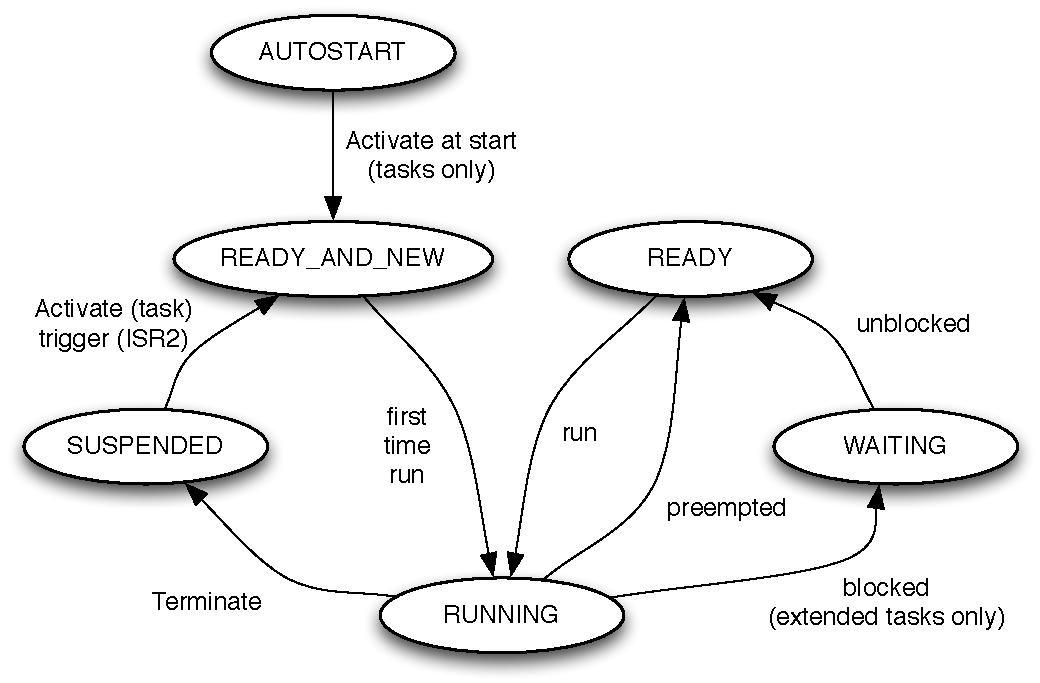
\includegraphics[width=4in]{pictures/states.pdf} 
   \caption{States of a process in Trampoline. AUTOSTART is the initial state of autostart tasks. SUSPENDED is the initial state of both non autostart tasks and ISR category 2.}
   \label{fig:states}
\end{figure} 


\section{The {\em idle} task}

The "idle" task is launched when no other task is currently running. It keeps the microprocessor doing nothing.\\
To be able to use specific platform capabilities (to put the microcontroler in stand by mode for example), this task is hardware specific (in \textit{machine/}). The taks is then able to quantify the microprocessor occupation.\\
GOIL doesn't produce anything about this idle task (unlike application(s) task(s)). The static part of the idle task descriptor is defined in \file{tpl_os_kernel.c} and we're be able to see that :
\begin{itemize}
\item the priority is 0
\item it's a basic task
\end{itemize}

%!TEX root = ./trampoline.tex

\chapter{Timing Protection Implementation}

The Timing Protection Implementation uses 2 timers. The first one is a {\em Free Running Timer} (FRT) which is used for {\em Time Frame}. The second one is a classical timer called {\em Timing Protection Timer} (TPT) which is used for \emph{Execution Time Budget}, \emph{Resource Locking Budget} and \emph{Interrupt Disabling Budget}.

\section{Low Level Functions}

These functions are provided by the {\em Board Support Package} and are used to manage the timers needed by the Timing Protection.

\subsection{FRT related functions}

\paragraph{\function{tpl_status tpl_start_frt(void)}} starts the FRT. On a microcontroller having a FRT that starts automatically when the system is powered on, this function does nothing but must be present since it is called by Trampoline in initialization stage. An error code is returned: {\em E\_OK} means no error, {\em E\_OS\_NOFUNC} means the FRT could not be started.

\paragraph{\function{tpl_status tpl_read_frt(tpl_tp_tick *out_value)}} write the current value of the FRT in \var{out_value}. An error code is returned: {\em E\_OK} means no error, {\em E\_OS\_NOFUNC} means the FRT could not be read.

\paragraph{\function{tpl_status tpl_elapsed_frt(tpl_tp_tick last_tick, tpl_tp_tick *out_value)}} write the number of ticks elapsed since \var{last_tick} in \var{out_value}. If the FRT has overflown/underflown between the time \var{last_tick} was get and the time \function{tpl_elapsed_frt} is called, \function{tpl_elapsed_frt} gives a correct value. An error code is returned: {\em E\_OK} means no error, {\em E\_OS\_NOFUNC} means the FRT could not be read.

\subsection{TPT related functions}

\paragraph{\function{tpl_status tpl_init_tpt(???)}} initializes the TPT. An error code is returned: {\em E\_OK} means no error, {\em E\_OS\_NOFUNC} means the TPT could not be initialized.

\paragraph{\function{tpl_status tpl_deinit_tpt(void)}} deinitializes the TPT. An error code is returned: {\em E\_OK} means no error, {\em E\_OS\_NOFUNC} means the TPT could not be deinitialized.

\paragraph{\function{tpl_status tpl_start_tpt(tpl_tp_tick delay)}} starts the TPT with an expiration delay equal to \var{delay} ticks. At that time, the \function{tpl_tpt_handler} function is called. An error code is returned: {\em E\_OK} means no error, {\em E\_OS\_NOFUNC} means the TPT could not be started because it is not initialized.

\paragraph{\function{tpl_status tpl_read_tpt(tpl_tp_tick *out_value)}} write the current value of the TPT in \var{out_value}. An error code is returned: {\em E\_OK} means no error, {\em E\_OS\_NOFUNC} means the TPT could not be read.

\paragraph{\function{tpl_status tpl_elapsed_tpt(tpl_tp_tick last_tick, tpl_tp_tick *out_value)}} write the number of ticks elapsed since \var{last_tick} in \var{out_value}. An error code is returned: {\em E\_OK} means no error, {\em E\_OS\_NOFUNC} means the TPT could not be read.

%!TEX root = ./trampoline.tex



%% HEAD SUPERTABULAR %%
\rowcolors{1}{light-gray}{white}
\newlength{\Li}\settowidth{\Li}{\textbf{Decimal}}
\newlength{\Liii}\settowidth{\Liii}{(bootstrap  )}
\newlength{\Lii}\settowidth{\Lii}{SCHEDULETABLE_AUTOSTART }
\tablefirsthead{ \textbf{Decimal Value} & \textbf{bit 5}  & \textbf{bit 4} & \textbf{bit 3} & \textbf{bit 2} & \textbf{bit 1} & \textbf{bit 0} & \textbf{Meaning} \\ \hline }
\tablehead{ \rowcolor{white} \rowcolors{1}{light-gray}{white} \textbf{Decimal Value} & \textbf{bit 5}  & \textbf{bit 4} & \textbf{bit 3} & \textbf{bit 2} & \textbf{bit 1} & \textbf{bit 0} & \textbf{Meaning} \\ \hline  }
\tabletail{ \hline } 
\tablelasttail{}


\chapter{Schedule Table Implementation}

Here is the files list :
\begin{itemize}
\item \file{tpl_as_schedtable.c} contains the API services.
\item \file{tpl_as_st_kernel.c} contains the kernel API services, \function{tpl_process_schedtable()} and \function{tpl_adjust_next_expiry_point()}
\item \file{tpl_as_action.c} contains \function{tpl_action_finalize_schedule_table()}
\item \file{tpl_as_definitions.h} contains the schedule table's states (SCHEDULETABLE\_STOPPED, SCHEDULETABLE\_BOOTSTRAP, SCHEDULETABLE\_AUTOSTART\_ABSOLUTE...)
\item \file{tpl_os_timeobj_kernel.c} contains \function{tpl_remove_time_obj()} which has been modified for the schedule table object.
\end{itemize}

The schedule table class diagram is shown in Figure \ref{fig:STobject} below.

\begin{figure}[H] %  figure placement: here, top, bottom, or page
   \centering
   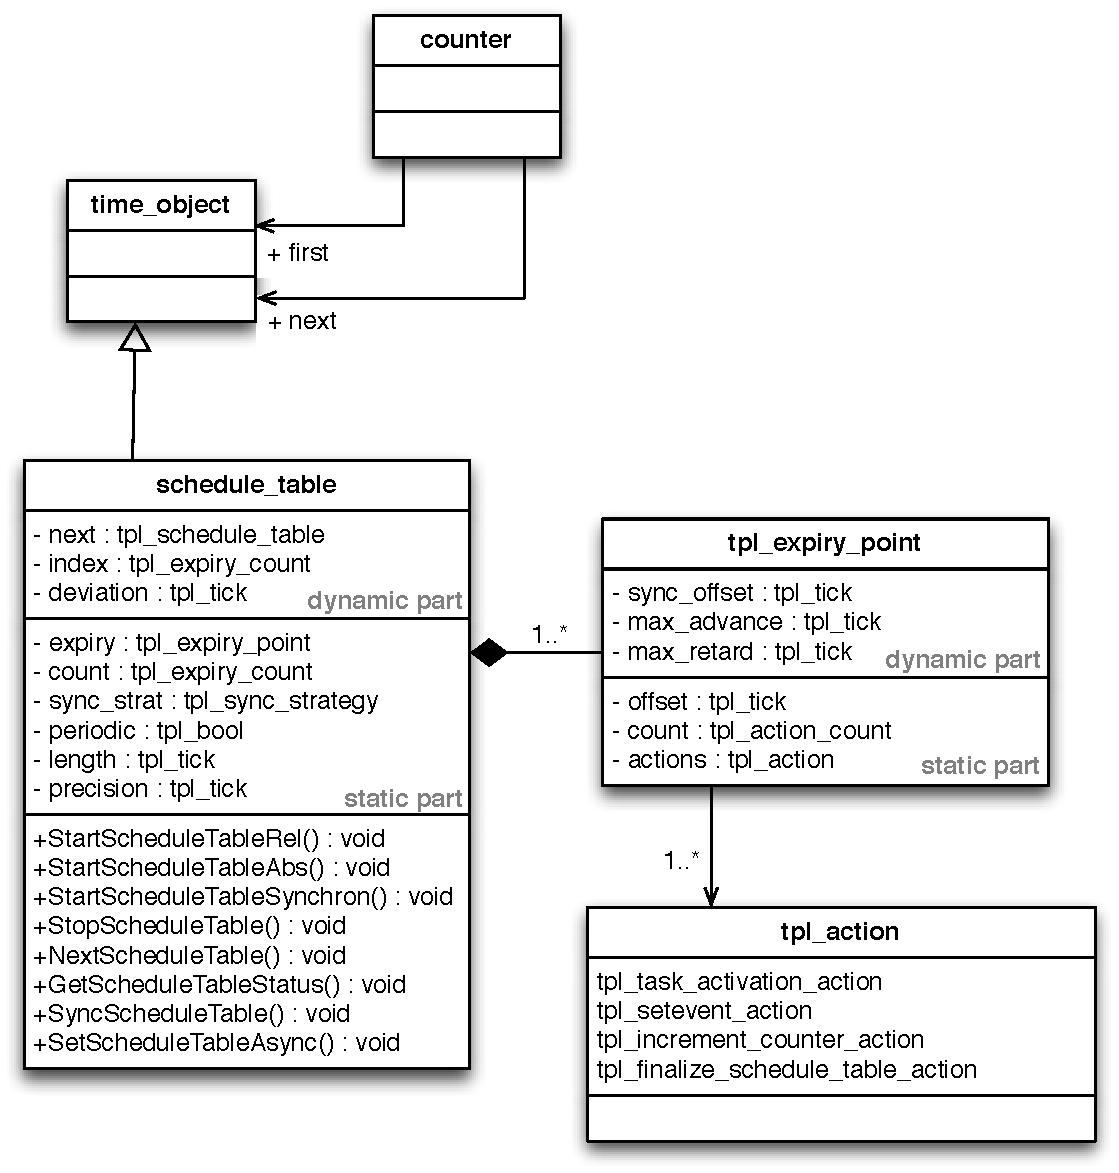
\includegraphics[scale=0.6]{pictures/STobject.pdf}  
   \caption{Schedule table class diagram}
   \label{fig:STobject}
\end{figure} 



\section{The States of a Schedule Table}

A schedule table always has a defined state. States include those found at page 42 of the AUTOSAR specifications 3.1 and others states used for internal management.

Indeed, \textbf{bit 1} is the "autostart" bit. It's used when autostarted schedule tables have been declared in the OIL file. Goil generates schedule tables with SCHEDULETABLE\_AUTOSTART\_X (X can be RELATIVE, ABSOLUTE or SYNCHRON) state. At startup (in \function{tpl_init_os()}), the system starts autostarted schedule tables and resets the \textbf{bit 1}.

\textbf{bit 4} is the "bootstrap" bit. It's used when the first expiry point of a schedule table is dated in more than \textbf{OsCounterMaxAllowedValue} ticks from the current date\footnote{As the \toreplace{offset} parameter of StartScheduleTableRel() cannot be greater than \textbf{OsCounterMaxAllowedValue} minus the \textbf{InitialOffset} of the schedule table (OS276), the first expiry point cannot be in more than \textbf{OsCounterMaxAllowedValue} ticks from the current date. Thus the "bootstrap" bit can set by StartScheduleTableAbs() only.}. It can happen when :
	\begin{itemize}
	\item the schedule table start (\toreplace{tick_val}) is after the current date and the first expiry point comes between the current date and \toreplace{tick_val}
	\item \toreplace{tick_val} is before the current date and the first expiry point comes after the current date
	\end{itemize}

Figure \ref{fig:bootstrapexample} below shows a bootstrap example for the first item.

\begin{figure}[H] %  figure placement: here, top, bottom, or page
   \centering
   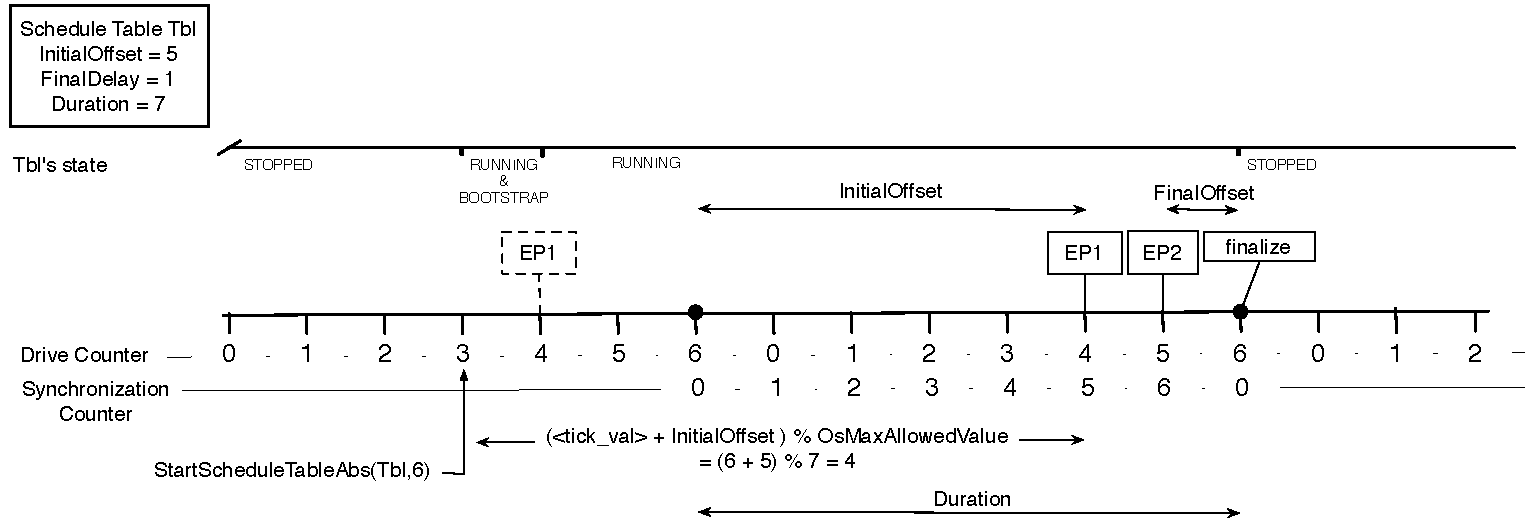
\includegraphics[scale=0.6]{pictures/BootstrapExample.pdf}  
   \caption{Bootstrap example}
   \label{fig:bootstrapexample}
\end{figure} 

\textbf{bit 5} is the "asynchronous" bit. It tells the system that the schedule table is in asynchronous mode.\\
Thus, the different states of a schedule table are described in Table \ref{schedtablestates} below.


\begin{table}[H]
\begin{center}
\topcaption{\textcolor{white}{q}States of a schedule table } % Latex is weird, the table goes on the next page without the "\textcolor{white}{q}"
\begin{supertabular}{p{\Li}|c|c|c|c|c|c|p{\Lii}|} 
0	& 0	& 0	& 0 	& 0	& 0	& 0	& SCHEDULETABLE_STOPPED  \\ 
1	& 0	& 0	& 0 	& 0	& 0	& 1	& SCHEDULETABLE_RUNNING  \\ 
5	& 0	& 0	& 0 	& 1	& 0	& 1	& SCHEDULETABLE_NEXT  \\  
9	& 0	& 0	& 1 	& 0	& 0	& 1	& SCHEDULETABLE_WAITING  \\  
13	& 0	& 0	& 1 	& 1	& 0	& 1	& SCHEDULETABLE_RUNNING_AND_SYNCHRONOUS \\ \hline \hline
6	& 0	& 0	& 0 	& 1	& 1	& 0	& SCHEDULETABLE_AUTOSTART _ABSOLUTE  \\ 
10	& 0	& 0	& 1 	& 0	& 1	& 0	& SCHEDULETABLE_AUTOSTART _RELATIVE  \\  
14	& 0	& 0	& 1 	& 1	& 1	& 0	& SCHEDULETABLE_AUTOSTART _SYNCHRON  \\  \hline \hline
16	& 0	& 1	& 0 	& 0	& 0	& 0	& SCHEDULETABLE_BOOTSTRAP \\ 
32	& 1	& 0	& 0 	& 0	& 0	& 0	& SCHEDULETABLE_ASYNC  \\ 
\end{supertabular} 
\end{center}
\label{schedtablestates}
\end{table}

Figure \ref{fig:STstates} shows how a schedule table goes from state to state.

\begin{figure}[H] %  figure placement: here, top, bottom, or page
   \centering
   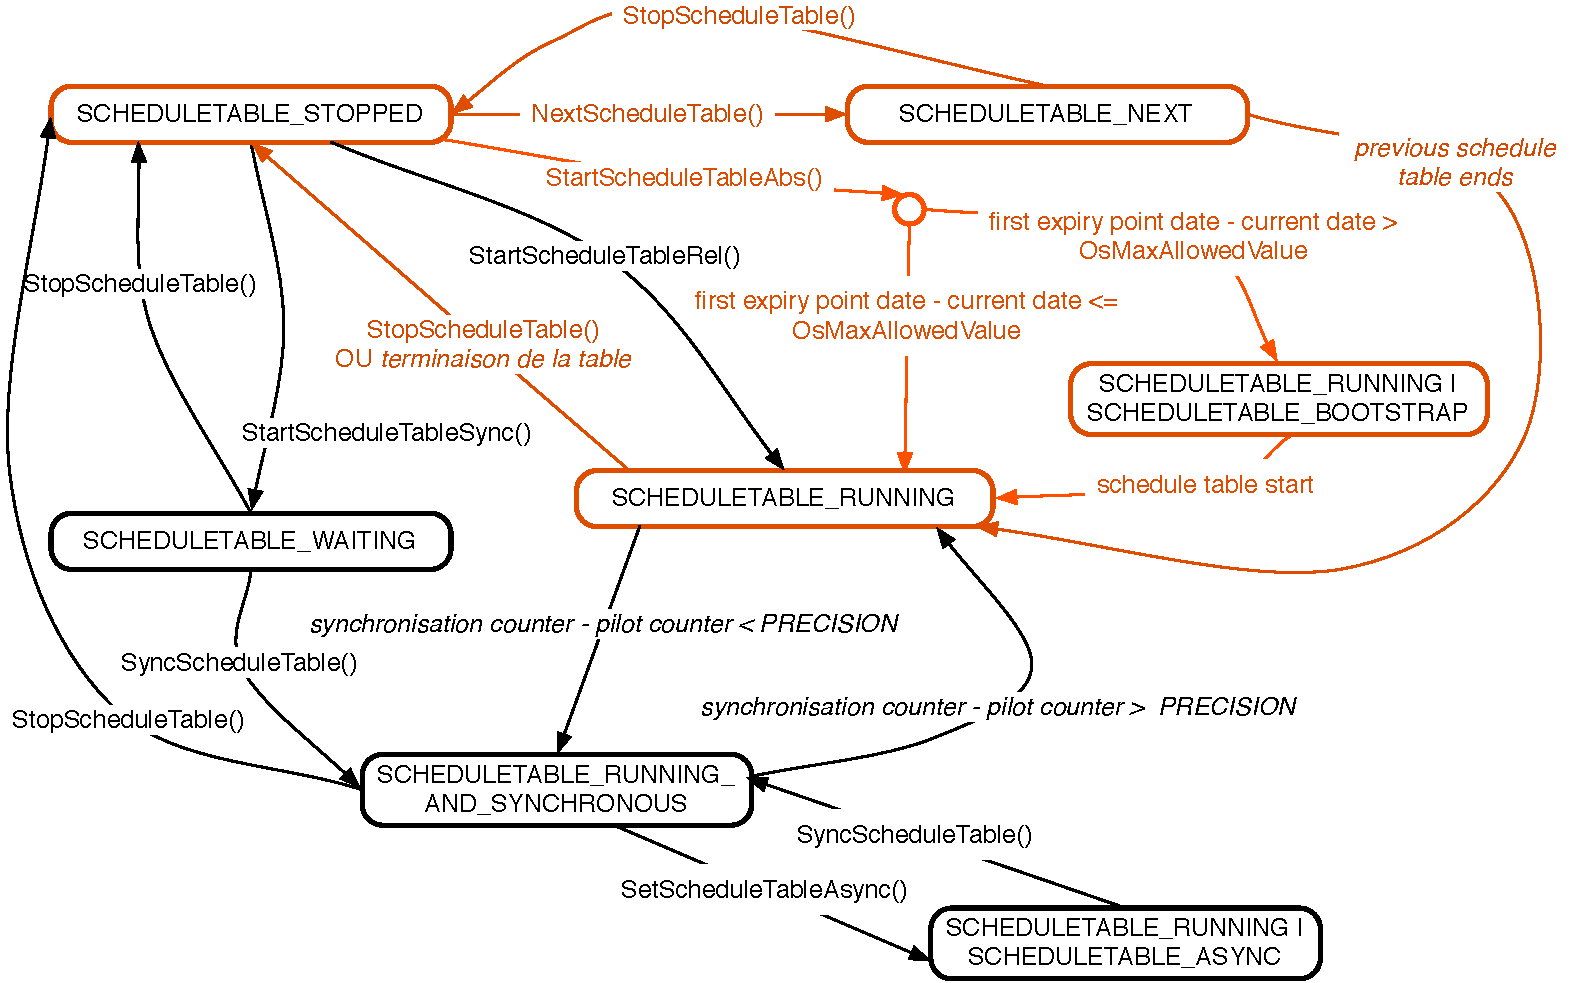
\includegraphics[scale=0.6]{pictures/STstates.pdf}  
   \caption{States of a schedule table in Trampoline.}
   \label{fig:STstates}
\end{figure} 
	
\section{Processing a Schedule Table}

In the same time of producing the schedule tables expiry points, GOIL adds one expiry point more than the number of expiry point delared in the OIL file : the "finalize" expiry point (see Figure \ref{fig:bootstrapexample}). Indeed, the RUNNING state of a "nexted" schedule table should be set at the finalize expiry point, thus, this expiry point has to be inserted. Moreover, for a periodic schedule table, the "finalize" expiry point helps to launch the first expiry point of the next period.

To process a \textbf{synchronized} schedule table, the schedule table's state has to be updated each expiry point and the next expiry point has to be adjusted according to the schedule table's deviation each epiry point too.

A schedule table is a time object, like an alarm. \function{tpl_processing_scheduletable()} is called by each expiry point (before activating a task, setting an event or finalizing a schedule table via \function{tpl_finalize_expiry_point()}) . The state machine of this function is shown in the Figure \ref{fig:STprocessingTplProcess}.

\begin{figure}[H] %  figure placement: here, top, bottom, or page
   \centering
   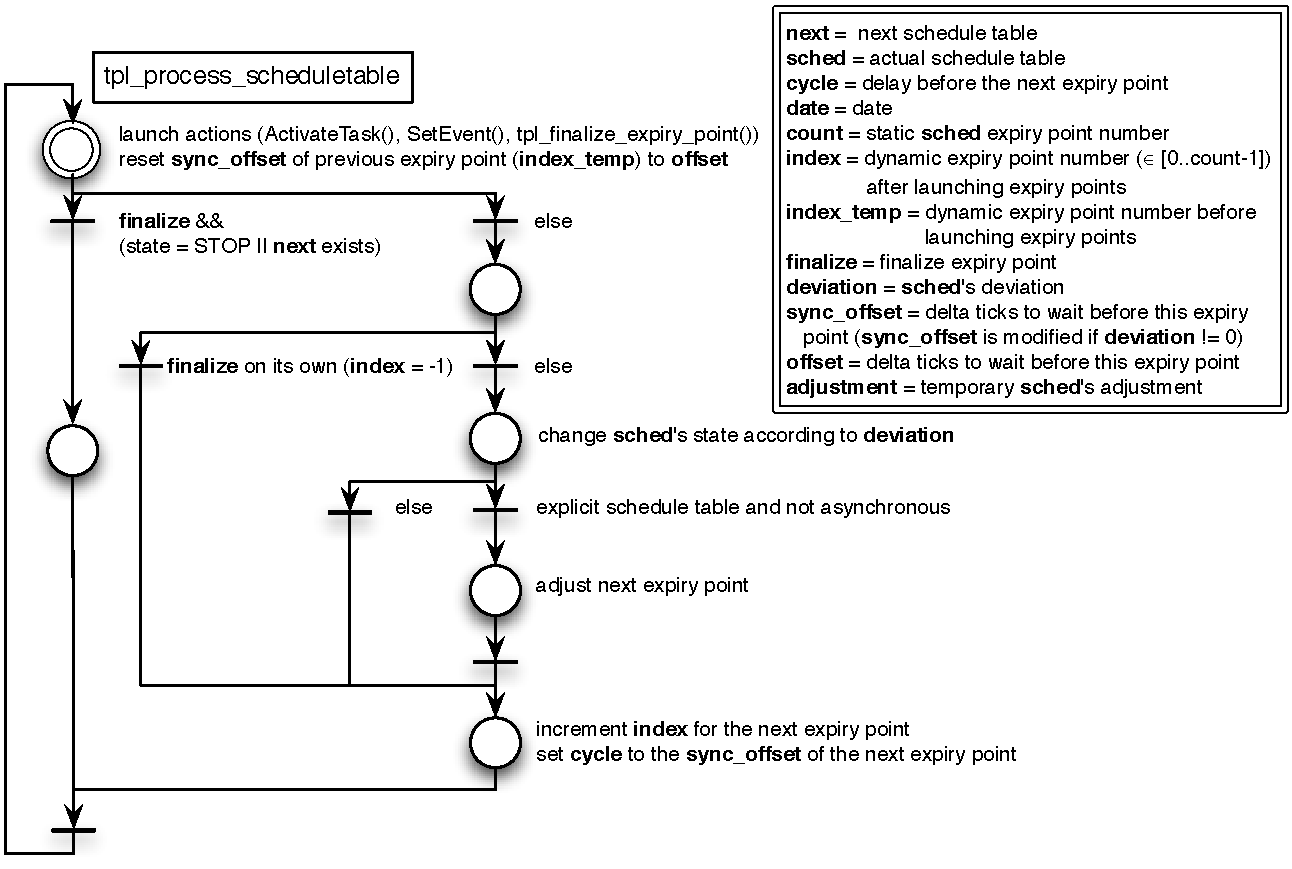
\includegraphics[scale=0.6]{pictures/STprocessingTplProcess.pdf}  
   \caption{tpl_process_scheduletable's state machine.}
   \label{fig:STprocessingTplProcess}
\end{figure} 

\begin{figure}[H] %  figure placement: here, top, bottom, or page
   \centering
   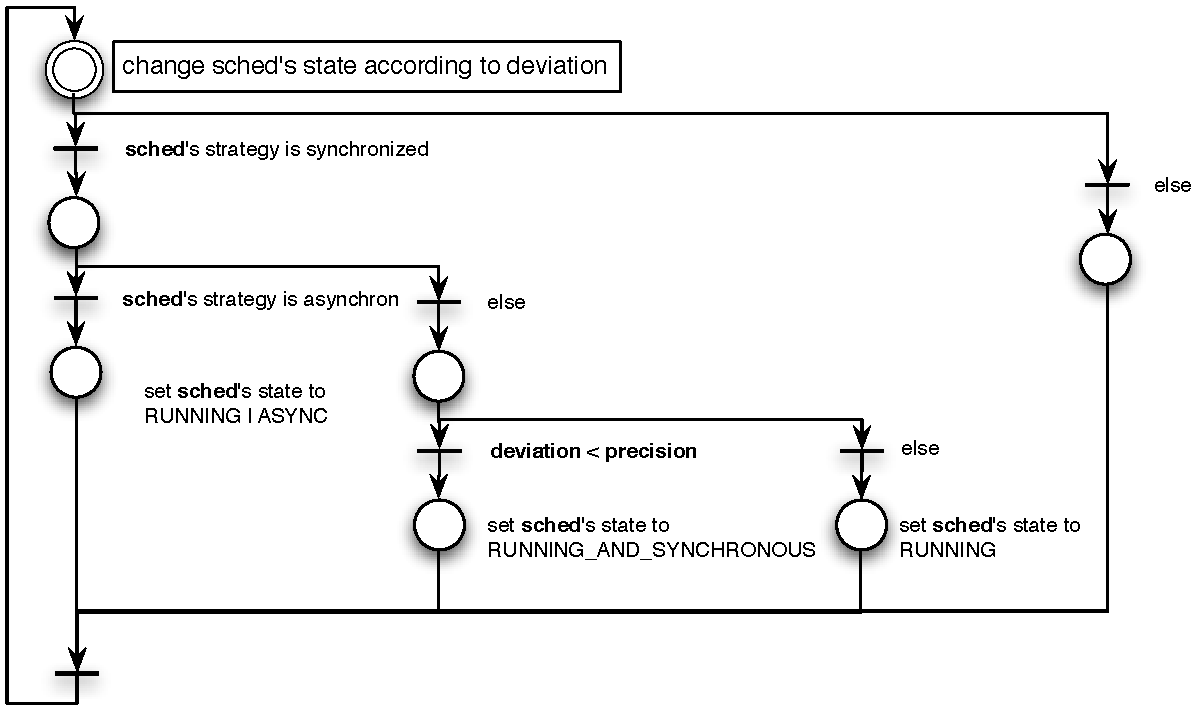
\includegraphics[scale=0.6]{pictures/STprocessingChangeState.pdf}  
   \label{fig:STprocessingChangeState}
\end{figure}

\begin{figure}[H] %  figure placement: here, top, bottom, or page
   \centering
   \includegraphics[scale=0.6]{pictures/STprocessingTplAdjust.pdf}  
   \label{fig:STprocessingTplAdjust}
\end{figure}

\function{tpl_finalize_expoiry_point()} state machine is shown in Figure \ref{fig:STprocessingTplFinalize} below.

\begin{figure}[H] %  figure placement: here, top, bottom, or page
   \centering
   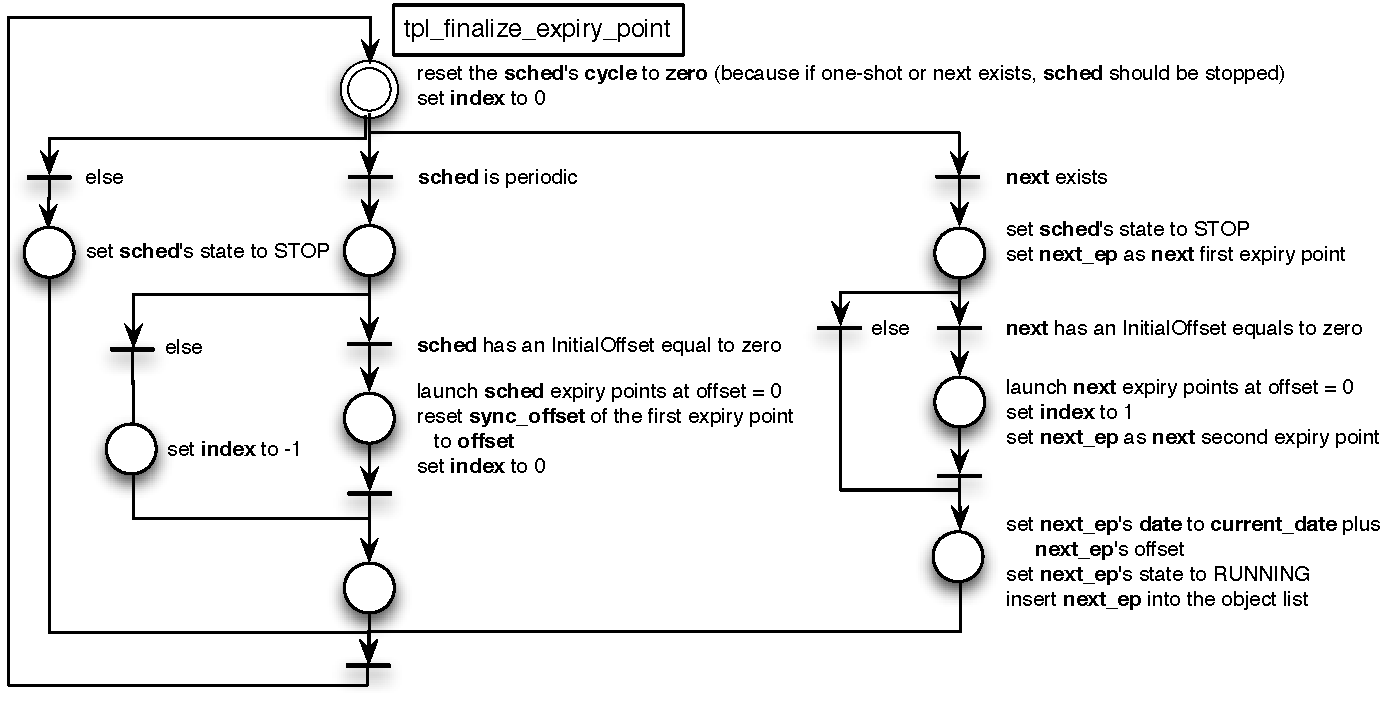
\includegraphics[scale=0.6]{pictures/STprocessingTplFinalize.pdf}  
   \caption{tpl_finalize_expiry_point's state machine.}
   \label{fig:STprocessingTplFinalize}
\end{figure} 

















%!TEX root = ./trampoline.tex

\chapter{The communication library}

\section{Internals}


%!TEX root = ./trampoline.tex

\chapter{System generation and compilation}

Trampoline is a static operating system. This means all the objects (tasks, ISR, ...) are known at compile time. This way, an application is made of tasks' code and ISRs' code, application data, and statically initialized descriptor for each object the operating system manages. A system generation tool, like \goil, generates these descriptors in C files from an application configuration described in OIL or in XML. After that the Trampoline source code, the generated files and the application source code are compiled and linked together to produce an executable file as shown in figure \ref{fig:buildtrampoline}.

\begin{figure}[htbp] %  figure placement: here, top, bottom, or page
   \centering
   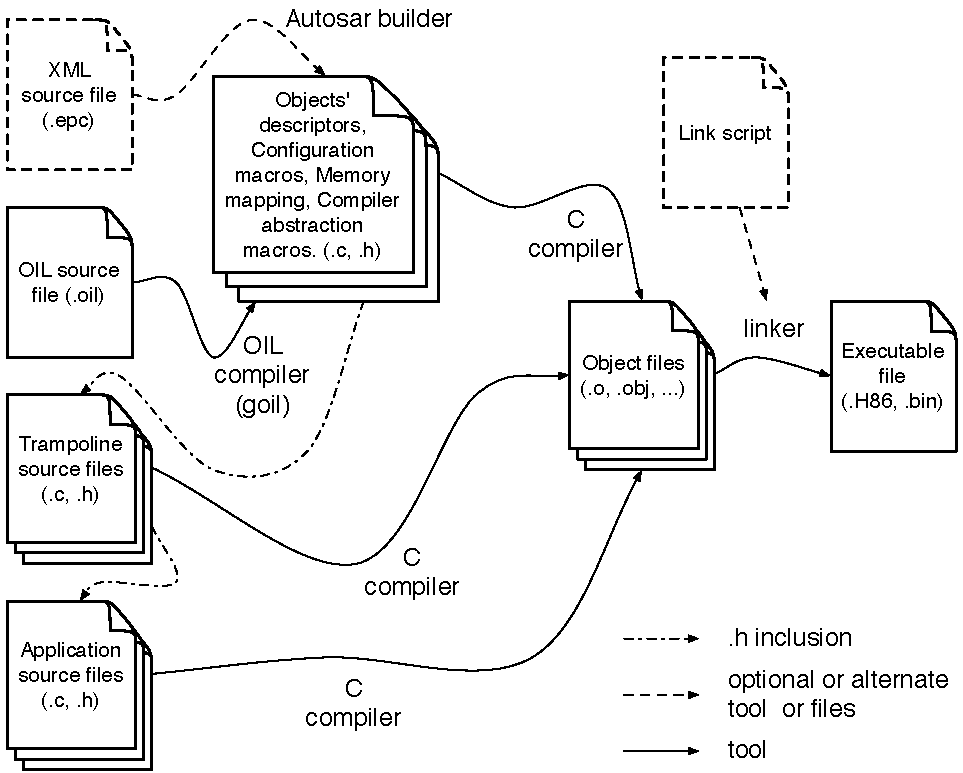
\includegraphics[width=4.5in]{pictures/buildProcess.pdf} 
   \caption{\textbf{Build process of an application with Trampoline.} Starting from the left, the .c and .h corresponding to the application description given in OIL (or XML) are generated by \goil\ (or another system generation tool, for instance an Autosar compliant one) and compiled using a C compiler. Trampoline source files are compiled too and include .h from the description for configuration purpose (see section \ref{sec:configmacros}). Application files are compiled and include .h files from Trampoline. All the object files are then linked together using an optional link script generated by \goil\ or provided with the application.}\label{fig:buildtrampoline}
\end{figure}

\section{The generated files}
\label{sec:generatedfiles}

The following files are generated by \goil\ from the OIL file or should be generated if you use a different system configuration tool. More information may be found in part \ref{part:goil}.

\rowcolors{1}{white}{light-gray}
\begin{longtableii}{l|p{3.5in}}{file}{File name}{Usage}

\lineii{tpl_app_define.h\index{tpl_app_define.h}}{This file contains all the configuration macros (see section \ref{sec:configmacros}) and is included in all the Trampoline files to trigger conditional compilation. \goil\ generates this file using the \file{tpl_app_define_h.goilTemplate} template file.}

\lineii{tpl_app_config.h\index{tpl_app_config.h}}{This file contains the declarations of the constants and functions required by the OSEK and Autosar standard (like OSMAXALLOWEDVALUE_x, OSTICKSPERBASE_x or OSMINCYCLE_x constants for counter x). \goil\ generates this file using the \file{tpl_app_config_h.goilTemplate} template file.}

\lineii{tpl_app_config.c\index{tpl_app_config.c}}{This file contains the definitions of the constants and functions required by the OSEK and Autosar standard and the definitions of object descriptors used by Trampoline (see section \ref{sec:structs}) \goil\ generates this file using the \file{tpl_app_config_c.goilTemplate} template file.}

\lineii{tpl_app_custom_types.h\index{tpl_app_custom_types.h}}{Some data types used by Trampoline are not statically defined. They are generated to fit size or performance criterions. For instance, the type used for a TaskType may be a byte if there is less than 256 tasks in the system and a word otherwise. This file defined these data types.}

\lineii{tpl_service_ids.h\index{tpl_service_ids.h}}{This file is generated only if Trampoline is compiled with service calls implemented using a system call. It contains all the identifiers of the services used by the application according to the configuration. \goil\ generates this file using the \file{tpl_service_ids_h.goilTemplate} template file.}

\lineii{tpl_dispatch_table.c\index{tpl_dispatch_table.c}}{This file is generated only if Trampoline is compiled with service calls implemented using a system call. It contains the dispatch table definition. See section \ref{sec:dispatchtable}. \goil\ generates this file using the \file{tpl_dispatch_table_c.goilTemplate} template file.}

\lineii{tpl_invoque.S\index{tpl_invoque.S}}{This file is generated only if Trampoline is compiled with service calls implemented using a system call. It contains the API functions for system services. See section \ref{sec:invoque}. The extension (here .S) may change according to the assembler used. \goil\ generates this file using the \file{tpl_invoque.goilTemplate} and \file{service_call.goilTemplate} template files.}

\lineii{MemMap.h\index{MemMap.h}}{This file is generated only if memory mapping is enabled. It contains macros for compiler abstraction memory mapping of functions and data as defined in the Autosar standard \cite{autosar31memorymapping}. \goil\ generates this file using the \file{MemMap_h.goilTemplate} template file.}

\lineii{Compiler.h\index{Compiler.h}}{This file is generated only if memory mapping is enabled. It contains macros for the compiler abstraction of functions and pointer qualifier as defined in the Autosar standard \cite{autosar31compilerabstraction}. \goil\ generates this file using the \file{Compiler_h.goilTemplate} template file.}

\lineii{Compiler_Cfg.h\index{Compiler_Cfg.h}}{This file is generated only if memory mapping is enabled. It contains macros for the compiler abstraction configuration as defined in the Autosar standard \cite{autosar31compilerabstraction}. \goil\ generates this file using the \file{Compiler_Cfg_h.goilTemplate} template file.}

\lineii{script.ld\index{script.ld}}{This file is generated only if memory mapping is enabled. It contains a link script to map the executable in the target memory. \goil\ generates this file using the \file{script.goilTemplate} template file.}

\end{longtableii}

The following sections give details about the content of these files.

\section{The Configuration Macros}
\label{sec:configmacros}

Trampoline can be compiled with various options. These options are controlled by setting the appropriate preprocessor configuration macros%
\index{Configuration macros}.
These macros are usually set by \goil
using the template found in \file{tpl_app_define_h.goilTemplate} file to produce the \file{tpl_app_define.h}\index{tpl_app_define.h} file that is included by the files of Trampoline. However, a different generation tool may be used and it should comply to the specification presented in the following tables. When Trampoline is compiled, the coherency and consistency of the configuration macros are checked, by using the preprocessor macros located in the \file{tpl_config_check.h} file, to ensure they correspond to a supported configuration.

3 kinds of configuration macros are used: boolean macros, numerical macros, symbol macros and string macros. Boolean macros may take 2 values: YES or NO. All macros should be defined, Trampoline does not use the \lstinline[language=C]{#ifdef} or \lstinline[language=C]{\#ifndef} scheme to limit the occurrences of unwanted misconfigurations except to prevent multiple inclusions of the same header file.

\subsection{Number of objects macros}

These macros gives the number of objects of each kind (tasks, ISRs, resources, \ldots) and other values. They are used in Trampoline to check the validity of the various identifiers and to define tables of the corresponding size:
 
\rowcolors{1}{white}{light-gray}
\begin{longtableiii}{l|l|p{3.1in}}{var}{Macro}{Kind}{Effect}
  \lineiii{\idxconfflag{PRIO_LEVEL_COUNT}}
  {Integer}
  {The number of priority levels used in the system.}
  \lineiii{\idxconfflag{TASK_COUNT}}
  {Integer}
  {The number of tasks (basic and extended) used in the system.}
  \lineiii{\idxconfflag{EXTENDED_TASK_COUNT}}
  {Integer}
  {The number of extended tasks used in the system.}
  \lineiii{\idxconfflag{ISR_COUNT}}
  {Integer}
  {The number of ISR category 2 used in the system.}
  \lineiii{\idxconfflag{ALARM_COUNT}}
  {Integer}
  {The number of alarms used in the system.}
  \lineiii{\idxconfflag{RESOURCE_COUNT}}
  {Integer}
  {The number of resources used in the system.}
  \lineiii{\idxconfflag{SEND_MESSAGE_COUNT}}
  {Integer}
  {The number of send messages used in the system.}
  \lineiii{\idxconfflag{RECEIVE_MESSAGE_COUNT}}
  {Integer}
  {The number of receive messages used in the system.}
  \lineiii{\idxconfflag{SCHEDTABLE_COUNT}}
  {Integer}
  {The number of schedule tables used in the system. This macros is only used when WITH_AUTOSAR is set to YES.}
  \lineiii{\idxconfflag{COUNTER_COUNT}}
  {Integer}
  {The number of counters used in the system. This macros is only used when WITH_AUTOSAR is set to YES.}
  \lineiii{\idxconfflag{APP_COUNT}}
  {Integer}
  {The number of OS applications used in the system. This macros is only used when WITH_AUTOSAR is set to YES.}
  \lineiii{\idxconfflag{TRUSTED_FCT_COUNT}}
  {Integer}
  {The number of trusted functions used in the system. This macros is only used when WITH_AUTOSAR is set to YES.}
  \lineiii{\idxconfflag{RES_SCHEDULER_PRIORITY}}
  {Integer}
  {The priority of the RES_SCHEDULER resource. This should be equal to the highest priority among the tasks.}
\end{longtableiii}

\subsection{Error Handling Macros}

Error handling related macros are used to configure what kind of error Trampoline checks and what extra processing is done when an error is encountered. The following macros are available:

\rowcolors{1}{white}{light-gray}
\begin{longtableiii}{l|l|p{2.5in}}{var}{Macro}{Kind}{Effect}
  \lineiii{\idxconfflag{WITH_OS_EXTENDED}}
  {Boolean}
  {When set to YES, Trampoline system services perform error checking on their arguments. \var{WITH_OS_EXTENDED} is set to YES with a \var{STATUS} = EXTENDED and is set to NO with a \var{STATUS} = BASIC in the oil OS object.}
  \lineiii{\idxconfflag{WITH_ERROR_HOOK}\label{sec:errorhook}}
  {Boolean}
  {When set to YES, the \function{ErrorHook()} function is called if an error occurs. \var{WITH_ERROR_HOOK} is set to YES/NO with a \var{ERRORHOOK} = TRUE/FALSE in the oil OS object.}
  \lineiii{\idxconfflag{WITH_USEGETSERVICEID}}
  {Boolean}
  {When set to YES, Trampoline system services store the id of the current service. This id may be retrieved in the \function{ErrorHook()} function by using the \function{OSErrorGetServiceId()} macro. \var{WITH_USEGETSERVICEID} is set to YES/NO with a \var{USEGETSERVICEID} = TRUE/FALSE in the oil OS object.}
  \lineiii{\idxconfflag{WITH_USEPARAMETERACCESS}}
  {Boolean}
  {When set to YES, Trampoline system services store the arguments of the current service. These arguments may be retrieved in the \function{ErrorHook()} function by using the ad-hoc access macros (see \ref{sec:errorhook}). \var{WITH_USEPARAMETERACCESS} is set to YES/NO with a \var{USEPARAMETERACCESS} = TRUE/FALSE in the oil OS object.}
  \lineiii{\idxconfflag{WITH_COM_ERROR_HOOK}}
  {Boolean}
  {When set to YES, the communication error hook is called when error occurs in the communication sub-system. This macro is only available when WITH_COM is set to true.}
  \lineiii{\idxconfflag{WITH_COM_USEGETSERVICEID}}
  {Boolean}
  {When set to YES, Trampoline/COM system services store the id of the current service. This id may be retrieved in the \function{COMErrorHook()} function by using the \function{COMErrorGetServiceId()} macro. \var{WITH_COM_USEGETSERVICEID} is set to YES/NO with a \var{COMUSEGETSERVICEID} = TRUE/FALSE in the oil COM object.}
  \lineiii{\idxconfflag{WITH_COM_USEPARAMETERACCESS}}
  {Boolean}
  {When set to YES, Trampoline/COM system services store the arguments of the current service. These arguments may be retrieved in the \function{COMErrorHook()} function by using the ad-hoc access macros (see \ref{sec:comerrorhook}). \var{WITH_COM_USEPARAMETERACCESS} is set to YES/NO with a \var{COMUSEPARAMETERACCESS} = TRUE/FALSE in the oil COM object.}
  \lineiii{\idxconfflag{WITH_COM_EXTENDED}}
  {Boolean}
  {When set to YES, Trampoline/COM system services perform error checking on their arguments. \var{WITH_COM_EXTENDED} is set to YES with a \var{COMSTATUS} = EXTENDED and is set to NO with a \var{COMSTATUS} = BASIC in the oil COM object.}
\end{longtableiii}

\subsection{Protection Macros}

Protection macros deal with protection facility provided by the Autosar standard. The following Macros are available:

\rowcolors{1}{white}{light-gray}
\begin{longtableiii}{l|l|p{2.9in}}{var}{Macro}{Kind}{Effect}
  \lineiii{\idxconfflag{WITH_MEMORY_PROTECTION}}
  {Boolean}
  {When set to YES, Trampoline enables the memory protection facility. This is only supported on some ports (MPC5510 and ARM9 at time of writing). Memory protection requires the memory mapping and the use of system call. \var{WITH_MEMORY_PROTECTION} is set to YES/NO with the MEMORY_PROTECTION attribute of MEMMAP object (see \ref{sec:memmap}) set to TRUE/FALSE.}
  \lineiii{\idxconfflag{WITH_TIMING_PROTECTION}}
  {Boolean}
  {When set to YES, Trampoline enables the timing protection facility. \var{WITH_TIMING_PROTECTION} is set to YES if the \var{AUTOSAR_SC} is 2 or 4 (see \ref{sec:autosarsc}) and a least one of the objects specifies a timing protection related attribute in the oil file.}
  \lineiii{\idxconfflag{WITH_PROTECTION_HOOK}\label{sec:protectionhook}}
  {Boolean}
  {When set to YES, Trampoline calls the ProtectionHook() with the appropriate argument when a protection fault occurs. \var{WITH_PROTECTION_HOOK} is set to YES with a \var{PROTECTIONHOOK} = TRUE in the oil OS object.}
  \lineiii{\idxconfflag{WITH_STACK_MONITORING}}
  {Boolean}
  {When set to YES, Trampoline enables the stack monitoring. Each time a context switch occurs, the stack pointer is checked. If the stack pointer is outside the stack zone of the process, a fault occurs. \var{WITH_STACK_MONITORING} is set to YES with a \var{STACKMONITORING} = TRUE in the oil OS object.}
\end{longtableiii}

\subsection{Hook call macros}

Hook call macros control whether a hook is called or not. The following Macros are available:

\rowcolors{1}{white}{light-gray}
\begin{longtableiii}{l|l|p{3.1in}}{var}{Macro}{Kind}{Effect}
  \lineiii{\idxconfflag{WITH_ERROR_HOOK}}
  {Boolean}
  {see \ref{sec:errorhook}}
  \lineiii{\idxconfflag{WITH_PRE_TASK_HOOK}}
  {Boolean}
  {When set to YES, each time a task is scheduled, the function PreTaskHook() is called.
  \var{WITH_PRE_TASK_HOOK} is set to YES/NO with a \var{PRETASKHOOK} = TRUE/FALSE
  in the oil OS object.}
  \lineiii{\idxconfflag{WITH_POST_TASK_HOOK}}
  {Boolean}
  {When set to YES, each time a task is descheduled, the function PostTaskHook() is called.
  \var{WITH_POST_TASK_HOOK} is set to YES/NO with a \var{POSTTASKHOOK} = TRUE/FALSE
  in the oil OS object.}
  \lineiii{\idxconfflag{WITH_STARTUP_HOOK}}
  {Boolean}
  {When set to YES, the function StartupHook() is called within the StartOS service.
  \var{WITH_STARTUP_HOOK} is set to YES/NO with a \var{STARTUPHOOK} = TRUE/FALSE
  in the oil OS object.}
  \lineiii{\idxconfflag{WITH_SHUTDOWN_HOOK}}
  {Boolean}
  {When set to YES, the function ShutdownHook() is called within the ShutdownOS service.
  \var{WITH_SHUTDOWN_HOOK} is set to YES/NO with a \var{SHUTDOWNHOOK} = TRUE/FALSE
  in the oil OS object.}
  \lineiii{\idxconfflag{WITH_PROTECTION_HOOK}}
  {Boolean}
  {see \ref{sec:protectionhook}}
\end{longtableiii}

\subsection{Miscellaneous macros}

Here are the other available macros:

\rowcolors{1}{white}{light-gray}
\begin{longtableiii}{l|l|p{2.6in}}{var}{Macro}{Kind}{Effect}
  \lineiii{\idxconfflag{WITH_USERESSCHEDULER}}
  {Boolean}
  {When set to YES, the RES_SCHEDULER resource is used by at least one process. \var{WITH_USERESSCHEDULER} is set to YES/NO with a \var{USERESSCHEDULER} = TRUE/FALSE
  in the oil OS object.}
  \lineiii{\idxconfflag{WITH_SYSTEM_CALL}}
  {Boolean}
  {When set to YES, services are called by the mean of a system call, also known as a software interrupt (see section \ref{sec:systemcall}).
  \var{WITH_SYSTEM_CALL} is set to YES/NO according to the target architecture and requires a memory mapping}
  \lineiii{\idxconfflag{WITH_MEMMAP}}
  {Boolean}
  {When set to YES, a memory mapping is used: A \file{MemMap.h} files giving the available memory segments is included and should be generated or provided by the user. \goil\ generates such a file.
  \var{WITH_MEMMAP} is set to YES/NO with a \var{MEMMAP} = TRUE/FALSE
  in the oil OS object.}
  \lineiii{\idxconfflag{WITH_COMPILER_SETTINGS}}
  {Boolean}
  {When set to YES, the compiler dependent Autosar macros are used: \file{Compiler.h} and \file {Compiler_Cfg.h} files are includes and should generated or provided by the user. \goil\ generates these  files if \var{MEMMAP} is TRUE and the \var{COMPILER} sub-attribute is set.}
  \lineiii{\idxconfflag{WITH_AUTOSAR}}
  {Boolean}
  {When set to YES, Trampoline contains additional system services, code and declarations related to the Autosar standard. For instance, the counter descriptor includes the counter type (hardware or software).
  \var{WITH_AUTOSAR} is set to YES/NO when at least an Autosar object is present in the system configuration (oil file for instance).}
  \lineiii{\idxconfflag{TRAMPOLINE_BASE_PATH}}
  {String}
  {The path to Trampoline root directory.}
  \lineiii{\idxconfflag{AUTOSAR_SC}}
  {Integer}
  {The Autosar scalability class\index{Scalability class} ranging from 0 to 4. 0 means OSEK}
  \lineiii{\idxconfflag{WITH_OSAPPLICATION}}
  {Boolean}
  {When set to YES, OS Application\index{OS Application} are used.}
  \lineiii{\idxconfflag{WITH_TRACE}}
  {Boolean}
  {When set to YES, the tracing of the operating system is enabled. Only available if WITH_TRACE is set to YES.}
  \lineiii{\idxconfflag{TRACE_TASK}}
  {Boolean}
  {When set to YES, task (de)scheduling events are traced. Only available if WITH_TRACE is set to YES.}
  \lineiii{\idxconfflag{TRACE_ISR}}
  {Boolean}
  {When set to YES, ISR category 2 (de)scheduling events are traced. Only available if WITH_TRACE is set to YES.}
  \lineiii{\idxconfflag{TRACE_RES}}
  {Boolean}
  {When set to YES, resources get and release are traced. Only available if WITH_TRACE is set to YES.}
  \lineiii{\idxconfflag{TRACE_ALARM}}
  {Boolean}
  {When set to YES, alarm activities are traced. Only available if WITH_TRACE is set to YES.}
  \lineiii{\idxconfflag{TRACE_U_EVENT}}
  {Boolean}
  {When set to YES, user events are traced. Only available if WITH_TRACE is set to YES.}
  \lineiii{\idxconfflag{TRACE_FORMAT}}
  {Symbol}
  {Trace format. A function named tpl_trace_format_\toreplace{trace_format} is expected. Only available if WITH_TRACE is set to YES.}
  \lineiii{\idxconfflag{TRACE_FILE}}
  {String}
  {File name where the trace is stored. Usable on Posix target only. Only available if WITH_TRACE is set to YES.}
  \lineiii{\idxconfflag{WITH_IT_TABLE}}
  {Boolean}
  {When set to YES, the external interrupts are dispatched using a table of fonction pointers.}
  \lineiii{\idxconfflag{WITH_COM}}
  {Boolean}
  {When set to YES, internal communication is used.}
  \lineiii{\idxconfflag{TPL_COMTIMEBASE}}
  {Integer}
  {The COMTIMEBASE expresses in nanoseconds.}
  \lineiii{\idxconfflag{WITH_COM_STARTCOMEXTENSION}}
  {Boolean}
  {When set to YES, the communication extension function is called.}
\end{longtableiii}

\section{Application configuration}

The application configuration is generated by \goil\ using the template found in \file{tpl_app_config_h.goilTemplate} file and \file{tpl_app_config_c.goilTemplate} file to produce the \file{tpl_app_define.h}\index{tpl_app_define.h} and \file{tpl_app_define.c}\index{tpl_app_define.c} files.

\subsection{Counter related constants declaration}

The \file{tpl_app_config.h} files contains the counters related constants: those of the SystemCounter\footnote{the default counter of an OSEK operating system} and those of the counters defined by the user. The SystemCounter constants are located in the generated files because the SystemCounter default attributes may be modified by the user in the OIL or XML file. The constants of a user defined counter are declared as follow:

\begin{lstlisting}[language=C]
extern CONST(tpl_tick, OS_CONST) OSTICKSPERBASE_<counter name>;
extern CONST(tpl_tick, OS_CONST) OSMAXALLOWEDVALUE_<counter name>;
extern CONST(tpl_tick, OS_CONST) OSMINCYCLE_<counter name>;
\end{lstlisting}

Where \toreplace{counter name} is obviously the name given to the counter in the confguration. For the SystemCounter, the following constants are declared:

\begin{lstlisting}[language=C]
extern CONST(tpl_tick, OS_CONST) OSTICKSPERBASE;
extern CONST(tpl_tick, OS_CONST) OSMAXALLOWEDVALUE;
extern CONST(tpl_tick, OS_CONST) OSMINCYCLE;
\end{lstlisting}

\subsection{Events definition}

The \file{tpl_app_config.c} file should contain the event mask definitions. For each event defined in the configuration, the following lines should appear:

\begin{lstlisting}[language=C]
#define API_START_SEC_CONST_UNSPECIFIED
#include "tpl_memmap.h"

#define <event name>_mask <mask value>
CONST(EventMaskType, AUTOMATIC) <event name> = <event name>_mask;

#define API_STOP_SEC_CONST_UNSPECIFIED
#include "tpl_memmap.h"
\end{lstlisting}

Where \toreplace{event name} is the name given to the event in the configuration and \toreplace{mask value} is the value set by the user in the configuration or, when set to AUTO, the value computed by the generation tool.

\subsection{Standard resources definition}

Standard resources need the definition of an identifier used to reference the resource in a system service (\cfunction{GetResource()} and \cfunction{ReleaseResource()}) and an instance of a \ctype{tpl_resource} structure (see \ref{sec:structtplresource}). This is done with the following definitions:

\begin{lstlisting}[language=C]
#define API_START_SEC_CONST_UNSPECIFIED
#include "tpl_memmap.h"

#define <resource name>_id <resource id>
CONST(ResourceType, AUTOMATIC) <resource name> = <resource name>_id;

#define API_STOP_SEC_CONST_UNSPECIFIED
#include "tpl_memmap.h"

#define OS_START_SEC_VAR_UNSPECIFIED
#include "tpl_memmap.h"

VAR(tpl_resource, OS_VAR) <resource name>_rez_desc = {
  /* ceiling priority of the resource */  <resource priority>,
  /* owner previous priority          */  0,
  /* owner of the resource            */  INVALID_PROC_ID,
#if WITH_OSAPPLICATION == YES
  /* OS Application id                */  <resource application id>,
#endif    
  /* next resource in the list        */  NULL
};

#define OS_STOP_SEC_VAR_UNSPECIFIED
#include "tpl_memmap.h"
\end{lstlisting}

Where \toreplace{resource name} is the name given to the resource in the configuration, \toreplace{resource priority} is the priority of the resource that is computed by the generation tool and is the maximum priority of the processes that use the resource and \toreplace{resource application id} is the identifier of the OS Application the resource belongs to. Since this field is protected by \var{WITH_OSAPPLICATION}, it may be leaved empty when no OS Application is used.

\toreplace{resource id} ranges from 0 to the number of standard resources minus 1. Once every standard resource descriptor is defined, a table gathering pointers to the resource descriptors and indexed by the resource id has to be defined. This table is used by system services to get the resource descriptor from the resource id. Suppose 3 standard resource, \var{motor1}, \var{motor2} and \var{dac} has been defined and RES_SCHEDULER is used, the table should be as follow:

\begin{lstlisting}[language=C]
#define OS_START_SEC_CONST_UNSPECIFIED
#include "tpl_memmap.h"
CONSTP2VAR(tpl_resource, AUTOMATIC, OS_APPL_DATA)
tpl_resource_table[RESOURCE_COUNT] = {
  &motor1_rez_desc,
  &motor2_rez_desc,
  &dac_rez_desc,
  &res_sched_rez_desc  
};
#define OS_STOP_SEC_CONST_UNSPECIFIED
#include "tpl_memmap.h"
\end{lstlisting}

\var{\&res_sched_rez_desc}, the pointer to the resource descriptor of RES_SCHEDULER should always be the last element of the table. If RES_SCHEDULER is not used, simply remove it from the table.

\subsection{Tasks definition}

Each task needs an identifier to reference a task un a system service (\cfunction{ActivateTask()}, \cfunction{ChainTask()}, \cfunction{GetTaskState()}, \cfunction{SetEvent()} and \cfunction{GetEvent()}) and the declaration of the task function. The following definitions should appear for each task:

\begin{lstlisting}[language=C]
#define API_START_SEC_CONST_UNSPECIFIED
#include "tpl_memmap.h"

#define <task name>_id <task id>
CONST(TaskType, AUTOMATIC) <task name> = <task name>_id;

#define API_STOP_SEC_CONST_UNSPECIFIED
#include "tpl_memmap.h"

#define APP_Task_<task name>_START_SEC_CODE
#include "tpl_memmap.h"

FUNC(void, OS_APPL_CODE) <task name>_function(void);

#define APP_Task_<task name>_STOP_SEC_CODE
#include "tpl_memmap.h"
\end{lstlisting}

Where \toreplace{task name} is the name given to the task in the configuration and \toreplace{task id} is the identifier of the task computed by the system generation tool. Task ids should range from 0 to the number of tasks minus 1. In addition, id allocation must start with extended tasks first and basic task after. In addition an instance of the static task descriptor must be provided:

\begin{lstlisting}[language=C]
#define OS_START_SEC_CONST_UNSPECIFIED
#include "tpl_memmap.h"
CONST(tpl_proc_static, OS_CONST) <task name>_task_stat_desc = {
  /* context                  */  <task name>_CONTEXT,
  /* stack                    */  <task name>_STACK,
  /* entry point (function)   */  <task name>_function,
  /* internal ressource       */  <internal resource>,
  /* task id                  */  <task name>_id,
#if WITH_OSAPPLICATION == YES
  /* OS application id        */  <application>,
#endif
  /* task base priority       */  <task priority>,
  /* max activation count     */  <task activation>,
  /* task type                */  <task type>
#if WITH_AUTOSAR_TIMING_PROTECTION == YES
  /* pointer to the timing
     protection descriptor    */  ,<timing protection>
#endif
};
#define OS_STOP_SEC_CONST_UNSPECIFIED
#include "tpl_memmap.h"
\end{lstlisting}

Where \toreplace{task name} is the name given to the task in the configuration. \toreplace{internal resource} mays be one of the following:

\begin{itemize}
\item a pointer to the internal resource descriptor (see \ref{sec:internalresource}) if an internal resource has been defined in the configuration;
\item a pointer to the scheduler internal resource if the task has been defined as non-preemptable in the configuration;
\item NULL if none of the above cases apply.
\end{itemize}

\toreplace{application} is the id of the OS Application the task belongs to when OS Application are used or, when they are not used, nothing at all. \toreplace{task priority} is the priority of the task as computed by the \sysgen. \toreplace{task activation} is the maximum number of task activation allowed as defined in the configuration. \toreplace{task type} may be EXTENDED or BASIC. \toreplace{timing protection} is a pointer to the timing protection descriptor or NULL if no timing protection is defined for the task.

Also an instance of the dynamic task descriptor must be provided:

\begin{lstlisting}[language=C]
#define OS_START_SEC_VAR_UNSPECIFIED
#include "tpl_memmap.h"

VAR(tpl_proc, OS_VAR) <task name>_task_desc = {
  /* resources                      */  NULL,
#if WITH_MEMORY_PROTECTION == YES
  /* if > 0 the process is trusted  */  <trusted count>,    
#endif /* WITH_MEMORY_PROTECTION */
  /* activate count                 */  0,
  /* task priority                  */  <task priority>,
  /* task state                     */  <task state>
#if WITH_AUTOSAR_TIMING_PROTECTION == YES
  /* activation allowed             */  ,TRUE
#endif
};

#define OS_STOP_SEC_VAR_UNSPECIFIED
#include "tpl_memmap.h"
\end{lstlisting}

Where \toreplace{task name} is the name given to the task in the configuration. \toreplace{trusted count} is 0 if the task belongs to a non trusted OS Application and 1 if the tasks belongs to a trusted OS Application. \toreplace{task priority} is the priority of the task as computed by the \sysgen. \toreplace{task state} is the initial state of the task and must be set to AUTOSTART or SUSPENDED.

If the task is an EXTENDED one, an event mask descriptor is added:

%\lstdefinelanguage[trampconf]{C}{morecomment=[s][\color{red}]{<}{>}}

\begin{lstlisting}[language=C]
VAR(tpl_task_events, OS_VAR) <task name>_task_evts = {
  /* event set  */ 0,
  /* event wait */ 0
};
\end{lstlisting}

Where \toreplace{task name} is the name given to the task in the configuration.


%!TEX root = ./trampoline.tex

\chapter{Ports details}

\section{PowerPC}

\subsection{System services} \label{sec:systemservices}

The PowerPC port uses the \asfct{sc} software interrupt to call system services \cite{mpc32bsc}. \asfct{sc} stands for System Call. It saves the current \reg{PC} in \reg{SRR0} register and the current \reg{MSR} in \reg{SRR1} register and jump to the System Call handler.

The id of the system service to call is given in the \reg{r0} register and \reg{r0} save and restore are added around. For instance, the following listing gives the \api{ActivateTask} service code. These function are generated from templates by goil (see \ref{sec:generatedfiles}) and are part of the {\em invoque} layer (see \ref{sec:invoque}):

\begin{lstlisting}[language=C]
  .global ActivateTask
ActivateTask:
  subi r1,r1,4                       /* make room on stack    */
  stw  r0,0(r1)                      /* save r0               */
  li   r0,OSServiceId_ActivateTask   /* load r0 with the id   */
  sc                                 /* system call           */
  lwz  r0,0(r1)                      /* restore r0            */
  addi r1,r1,4                       /* restore stack         */
  blr                                /* return                */
  
  .type ActivateTask,@function
  .size ActivateTask,$$-ActivateTask
\end{lstlisting}

When the System Call begin execution, the process stack has the mapping depicted in figure \ref{fig:stackbeginningSC}.

\begin{figure}[htbp] %  figure placement: here, top, bottom, or page
\begin{minipage}{0.5\textwidth}
    \centering
  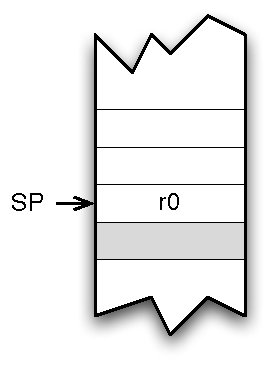
\includegraphics[scale=.6]{pictures/PStackAfterInvoque} 
\end{minipage}
\begin{minipage}{0.5\textwidth}
   \caption{Process stack mapping at the beginning of the System Call handler. The grayed zone represents an unknown content depending on from where the service was called.}\label{fig:stackbeginningSC}
\end{minipage}
\end{figure}

\subsection{Dispatching the service call}

The System Call handler is usually located in the \hex{0C00} exception handler but, depending on the CPU kind, it may be located elsewhere. Since the available memory for the interrupt or exception handler may vary, a jump is made to the \cfunction{tpl_sc_handler}.%:

%\begin{lstlisting}
%  .section  .SC_vector  CODE_ACCESS_RIGHT
%tpl_sc_vector:
%  b   tpl_sc_handler
%
%  .section  .SC_handler CODE_ACCESS_RIGHT
%\end{lstlisting}

\cfunction{tpl_sc_handler} performs the following tasks:
\begin{penum}
\item saves additional registers to be able to work
\item disables memory protection
\item switches to kernel stack if needed
\item calls the service
\item performs a context switch if needed and programs the MPU.
\item switches back to the process stack if needed
\item enable memory protection
\item restore registers
\item get back to the process
\end{penum}

\note{Currently the PowerPC port does not support tasks that use floating point registers}

\subsubsection{Saving additional registers}

The following registers are saved: \var{lr}, \var{cr}, \var{r11} and \var{r12}. In fact, it should be not necessary to save \var{r11} and \var{r12} because these registers are volatile as defined in the PowerPC EABI \cite{PPCeabi} but we prefer a conservative approach. Register saving is done by the following code at start of the \cfunction{tpl_sc_handler} and the mapping of the process stack is depicted at figure \ref{fig:stackSavingSC}:

\begin{lstlisting}[language=C]
  subi  r1,r1,PS_FOOTPRINT  /* Make room on stack */

  stw   r11,PS_R11(r1)      /* Save r11           */
  stw   r12,PS_R12(r1)      /* Save r12           */
  mflr  r11
  stw   r11,PS_LR(r1)       /* Save lr            */
  mfcr  r11
  stw   r11,PS_CR(r1)       /* Save cr            */
\end{lstlisting}

\begin{figure}[htbp] %  figure placement: here, top, bottom, or page
\begin{minipage}{0.5\textwidth}
    \centering
  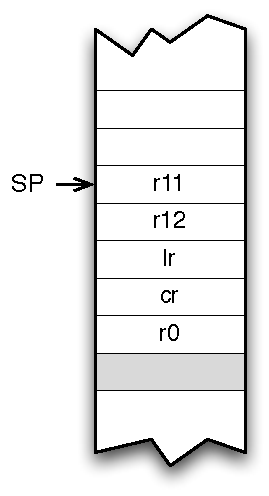
\includegraphics[scale=.6]{pictures/PStackAfterSCSaving} 
\end{minipage}
\begin{minipage}{0.5\textwidth}
   \caption{Process stack mapping after additional registers have been saved by the beginning of the System Call handler.}\label{fig:stackSavingSC}
\end{minipage}
\end{figure}

\subsubsection{Disabling memory protection}

This part of the dispatch layer is done in the \function{tpl_enter_kernel} function and is assembled only if \var{WITH_MEMORY_PROTECTION} is set to YES. After saving the \var{lr}, the \function{tpl_kernel_mp} function is called and does the actual job. At last \var{lr} is restored.

\begin{lstlisting}[language=C]
#if WITH_MEMORY_PROTECTION == YES
  /*
   * Switch to kernel mem protection scheme
   */
  subi  r1,r1,4
  mflr  r11
  stw   r11,0(r1)       /* save lr on the current stack */
  bl    tpl_kernel_mp   /* disable memory protection    */
  lwz   r11,0(r1)       /* restore lr                   */
  mtlr  r11
  addi  r1,r1,4
#endif
\end{lstlisting}

\subsubsection{Switching to the kernel stack}

Once the dispatch layer has saved the registers it uses and has switched to the kernel memory protection scheme, it switches to the kernel stack. However the kernel stack could used already because a call to a \function{PreTaskHook} or a \function{PostTaskHook} is done on the kernel stack and such a hook may call a service. So the dispatch layer is reentrant. The number of reentrant calls is counted by the \var{tpl_reentrancy_counter}. In addition the process stack pointer (\var{r1}), \var{SRR0} and \var{SRR1} are saved in the kernel stack. The kernel stack mapping is shown in figure \ref{fig:kernelstackmapping}. For a reentrant call, the same frame is build over the current one. The switch to the kernel stack is done as follow:

\begin{lstlisting}[language=C]
  /*
   * Check the reentrency counter value and increment it
   * if the value is 0 before the inc, then we switch to
   * the system stack.
   */
  lis   r11,TPL_HIG(tpl_reentrancy_counter)
  ori   r11,r11,TPL_LOW(tpl_reentrancy_counter)
  lwz   r12,0(r11)    /* get the value of the counter */
  cmpwi r12,0
  addi  r12,r12,1
  stw   r12,0(r11)
  bne   no_stack_change
  
  /*
   * Switch to the kernel stack
   *
   * Get the pointer to the bottom of the stack
   */  
  lis   r11,TPL_HIG(tpl_kernel_stack_bottom)
  ori   r11,r11,TPL_LOW(tpl_kernel_stack_bottom)
  stw   r1,KS_SP-KS_FOOTPRINT(r11)  /* save the sp of the caller */
  mr    r1,r11                      /* set the kernel stack      */
  
no_stack_change:
  /*
   * make space on the stack to call C functions
   */
  subi  r1,r1,KS_FOOTPRINT
\end{lstlisting}

\begin{figure}[htbp] %  figure placement: here, top, bottom, or page
\begin{minipage}{0.5\textwidth}
    \centering
  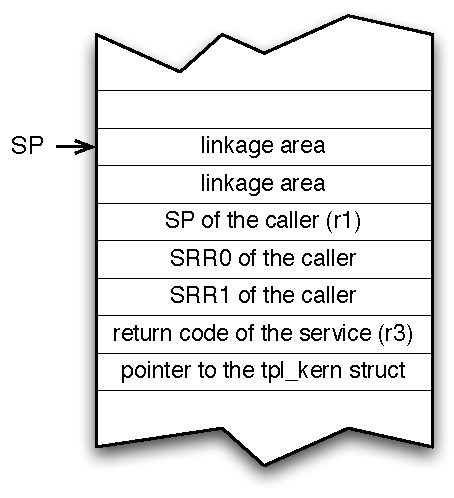
\includegraphics[scale=.6]{pictures/KStackMapping} 
\end{minipage}
\begin{minipage}{0.5\textwidth}
  \caption{Kernel stack mapping after allocation.}\label{fig:kernelstackmapping}
\end{minipage}
\end{figure}

\subsubsection{Calling the service}

Since the registers used to pass parameters to a function, that is \reg{r3} to \reg{r10} as documented in \cite{PPCeabi}, have not been changed until now, calling the function that implements the service respects the register usage conventions.

The first thing to do is to get the function pointer corresponding to the service id. The service id is in \reg{r0} as explained in \ref{sec:systemservices} and is used as an index to the \var{tpl_dispatch_table}.

\begin{lstlisting}[language=C]
  slwi  r0,r0,2                           /* compute the offset    */
  /*
   * load the ptr to the dispatch table
   */
  lis   r11,TPL_HIG(tpl_dispatch_table)     
  ori   r11,r11,TPL_LOW(tpl_dispatch_table)
  lwzx  r11,r11,r0                  /* get the ptr to the service  */
  mtlr  r11                         /* put it in lr for future use */
\end{lstlisting}

The second thing to do is to reset the \var{tpl_need_switch} flag that triggers a context switch. This flag (a byte) is located in the \var{tpl_kern} kernel struct. This is done as follow:

\begin{lstlisting}[language=C]
  lis   r11,TPL_HIG(tpl_kern)
  ori   r11,r11,TPL_LOW(tpl_kern)
  stw   r11,KS_KERN_PTR(r1)        /* save the ptr for future use  */
  li    r0,NO_NEED_SWITCH
  stb   r0,20(r11)
\end{lstlisting}

In the future \var{tpl_kern} will be reused, so its address is saved in the kernel stack.

Then, to allow reentrancy for a service call in a hook, the \reg{RI} bit of the \reg{MSR} is set to 1. Without that, a \asfct{sc} cannot be  properly executed.

\begin{lstlisting}[language=C]
  mfmsr r11
  ori   r11,r11,RI_BIT_1
  mtmsr r11
\end{lstlisting}

At last, the service is called:

\begin{lstlisting}[language=C]
  blrl
\end{lstlisting}

\subsubsection{Context switch}

The \var{tpl_need_switch} flag that as been possibly modified by the service is now checked to do a context switch if needed.

\begin{lstlisting}[language=C]
  lwz   r11,KS_KERN_PTR(r1) /* get back the tpl_kern address */
  lbz   r12,20(r11)         /* get the tpl_need_switch flag  */
  andi. r0,r12,NEED_SWITCH  /* check if a switch is needed   */
  beq   no_context_switch
\end{lstlisting}

A context switch is performed in 3 steps. The first one is the context save of the process that loses the CPU. This step is optional because if the service was a \api{TerminateTask} or a \api{ChainTask}, the context needs not to be saved. This information is in the \var{tpl_need_switch} flag. Before doing the actual context save, the return value of the service must be saved in the proper location of the kernel stack. The \cfunction{tpl_save_context} function will read it from this location and expects a pointer to the context saving area or the process in \reg{r3}. \var{s_old}, the address of the context saving area, is in another member of \var{tpl_kern}. At the end, the \var{tpl_kern} address is reread because \reg{r11} has been destroyed in \cfunction{tpl_save_context}. 

\begin{lstlisting}[language=C]
  stw   r3,KS_RETURN_CODE(r1) /* save the return value             */
  andi. r0,r12,NEED_SAVE      /* r12 contains tpl_need_switch      */
  beq   no_save
  lwz   r3,0(r11)             /* r11 contains the tpl_kern address */
  bl    tpl_save_context      /* and s_old is put into r3          */
  lwz   r11,KS_KERN_PTR(r1)   /* get back tpl_kern address         */
\end{lstlisting}

The second step consists in loading the configuration of memory protection for the process that get the CPU by calling the \cfunction{tpl_set_process_mp} function. This function expects the id of the process in \reg{r3}. Again this id is located in member \var{proc_id} of \var{tpl_kern}. This is done only if \var{WITH_MEMORY_PROTECTION} is \var{YES}. 

\begin{lstlisting}[language=C]
#if WITH_MEMORY_PROTECTION == YES
  lwz   r3,16(r11) /* get the id of the process which get the cpu  */
  bl    tpl_set_process_mp     /* set the memory protection scheme */
#endif
\end{lstlisting}

The third step loads the context of the process that get the CPU. The address of \var{tpl_kern} is loaded into \reg{r11} because it has been destroyed in \cfunction{tpl_set_process_mp}, \var{s_running}, the address of the context saving area of the current process is loaded into \reg{r3} and \cfunction{tpl_load_context} is called. At last, \reg{r3} is restored.

\begin{lstlisting}[language=C]
  lwz   r11,KS_KERN_PTR(r1)
  lwz   r3,4(r11)                    /* get s_running              */
  bl    tpl_load_context
  lwz   r3,KS_RETURN_CODE(r1)
\end{lstlisting}

\subsubsection{Switching back to the process stack}

At this stage, the \reg{SRR0} and \reg{SRR1} registers saved in the kernel stack are restored. The space reserved in the kernel stack is freed. The reentrancy counter is decremented and the stack switches to the process stack if the reentrancy counter is 0.

\begin{lstlisting}[language=C]
  lwz   r11,KS_SRR0(r1)
  mtspr spr_SRR0,r11
  lwz   r11,KS_SRR1(r1)
  mtspr spr_SRR1,r11

  addi  r1,r1,KS_FOOTPRINT       /*  free back space on the stack  */
  
  /*
   * The reentrency counter is decremented. If it reaches
   * 0, the process stack is restored
   */
  lis   r11,TPL_HIG(tpl_reentrancy_counter)
  ori   r11,r11,TPL_LOW(tpl_reentrancy_counter)
  lwz   r12,0(r11)    /*  get the value of the counter */
  subi  r12,r12,1
  stw   r12,0(r11)
  cmpwi r12,0
  bne   no_stack_restore

  /*  Restore the execution context of the caller
      (or the context of the task/isr which just got the CPU)      */
  lwz   r1,KS_SP-KS_FOOTPRINT(r1)   /*  Restore the SP and switch
                                        back to the process stack  */
\end{lstlisting}

\subsubsection{Enabling memory protection}

Then, if memory protection is used, the user scheme is reenabled. The actual works depends on the kind of MPU and is done in \cfunction{tpl_user_mp}.

\begin{lstlisting}[language=C]
#if WITH_MEMORY_PROTECTION == YES
  subi  r1,r1,4
  mflr  r11
  stw   r11,0(r1)   /* save lr on the current stack  */
  bl    tpl_user_mp /* Enable the memory protection  */
  lwz   r11,0(r1)   /* restore lr                    */
  mtlr  r11
  addi  r1,r1,4
#endif
\end{lstlisting}

\subsubsection{Restoring registers}

Registers saved at stage 1 on the process stack are restored an the stack is freed.

\begin{lstlisting}[language=C]
  lwz   r11,PS_CR(r1)
  mtcr  r11
  lwz   r11,PS_LR(r1)
  mtlr  r11
  lwz   r12,PS_R12(r1)
  lwz   r11,PS_R11(r1)

  addi  r1,r1,PS_FOOTPRINT
\end{lstlisting}

\subsubsection{Getting back to the process}

At last, the dispatch layer is exited using a \asfct{rfi}.

\begin{lstlisting}[language=C]
  rfi                                 /* return from interrupt */
\end{lstlisting}

\subsection{Interrupt handler}

\subsection{The CallTrustedFunction service}

The \api{CallTrustedFunction} service is implemented by the \cfunction{tpl_call_trusted_function_service} function. This function is a special case of service because the kernel stack and the process stack have to be modified. In addition, an \api{ExitTrustedFunction} service is implemented to restore the process stack when the trusted function exits. Both services have to be written in assembly language since C does not allow to explicitely modify the stack.

\cfunction{tpl_call_trusted_function_service} performs the following steps:

\begin{penum}
\item check the trusted function id is within the allowed range
\item increment the trusted counter of the calling process
\item build a frame on the process stack to store the registers pushed by a service call except for \reg{r0} and for \reg{SRR0} and \reg{SRR1}; put the address of \api{ExitTrustedFunction} in the \reg{lr} location in the process stack; save \reg{SRR0} and \reg{SRR1} in the process stack
\item get the trusted function address and put it in \reg{SRR0}
\item go back to the dispatch layer
\end{penum}

\subsubsection{Checking the trusted function id}

The id of the trusted function is checked to avoid to call a function at an arbitrary address.

\begin{lstlisting}[language=C]
  mov   r11,r3               /* save r3 in r11 b/c it will be destroyed    */
  cmpw  r3,TRUSTED_FCT_COUNT /* check the id of the trusted function       */
  ori   r3,r0,E_OS_SERVICEID /* E_OS_SERVICEID return code                 */
  bge   invalid_trusted_fct_id
  mov   r3,r11               /* restore r3 if the trusted function id ok   */
\end{lstlisting}

\subsubsection{Incrementing the trusted counter}

The trusted counter of the process is incremented each time a trusted function is called. When the trusted counter is $>0$, the process is trusted. In such a case, the dispatch layer does not enable memory protection when scheduling the process so it has an unlimited access to the whole addressing space.

\begin{lstlisting}[language=C]
  lwz   r11,KS_KERN_PTR(r1)   /* get the ptr to tpl_kern                  */
  lwz   r11,12(r11)           /* get the ptr to the runnning process desc */
  lwz   r12,4(r11)            /* get trusted_count member                 */
  addi  r12,r12,1             /* increment it                             */
  stw   r12,4(r11)            /* put it back in the process desc          */
\end{lstlisting}

\subsubsection{Building the frame}

The frame is used to store the calling context of the trusted function and is shown in figure \ref{fig:tfstackmapping}. The following code builds this frame:

\begin{lstlisting}[language=C]
  /*
   * First get back the process stack pointer
   */
  lwz   r11,KS_SP(r1)
  /*
   * Make room to prepare the call of the trusted function
   */
  subi  r11,r11,PS_TRUSTED_FOOTPRINT_IN
  /*
   * store ExitTrustedFunction as the return address
   */
  lis   r12,TPL_HIG(ExitTrustedFunction)
  ori   r12,r12,TPL_LOW(ExitTrustedFunction)
  stw   r12,PS_LR(r11)
  /*
   * Update the stack pointer
   */
  stw   r11,KS_SP(r1)
  /*
   * second get back SRR0 and SRR1 and save them to the process stack
   */
  lwz   r12,KS_SRR0(r1)
  stw   r12,PS_SRR0_IN(r11)
  lwz   r12,KS_SRR1_IN(r1)
  stw   r12,PS_SRR1(r11)
\end{lstlisting}

\begin{figure}[htbp] %  figure placement: here, top, bottom, or page
\begin{minipage}{0.65\textwidth}
    \centering
  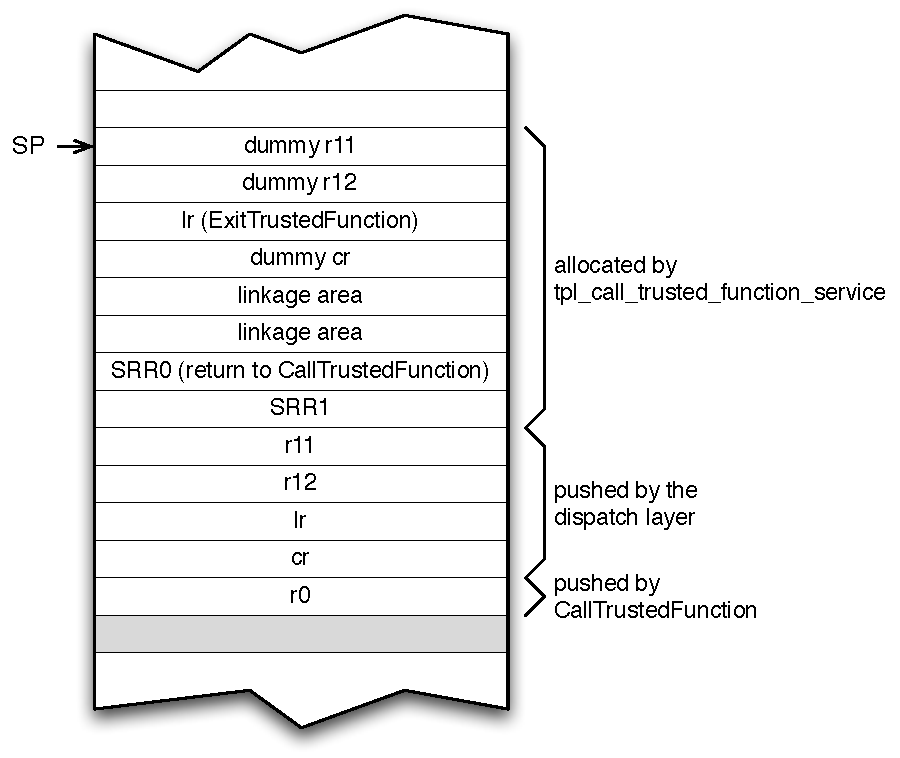
\includegraphics[scale=.6]{pictures/TFStack1} 
\end{minipage}
\begin{minipage}{0.35\textwidth}
  \caption{Process stack mapping at the end of \cfunction{tpl_call_trusted_function_service}. \reg{r0}, at the bottom of the stack has been pushed by CallTrustedFunction. \reg{cr} to \reg{r11} has been pushed by the dispatch layer. \reg{SRR0} and \reg{SRR1} are saved here by \cfunction{tpl_call_trusted_function_service} to be able to go back to the calling process. Above, the linkage area allows the trusted function to call functions. Above, a frame that will be used by the dispatch layer to restore an execution context for the trusted function is built.}\label{fig:tfstackmapping}
\end{minipage}
\end{figure}

\subsubsection{Setting the trusted function address}

The \reg{SRR0} saved by the dispatch layer after the \api{CallTrustedFunction} is changed to the address of the trusted function. This way, instead of returning to the caller, the trusted function will be executed.

\begin{lstlisting}
  lis   r11,TPL_HIG(tpl_trusted_fct_table)
  ori   r11,r11,TPL_LOW(tpl_trusted_fct_table)
  slwi  r0,r3,2
  lwzx  r12,r11,r0
  stw   r12,KS_SRR0(r1)
\end{lstlisting}

\subsubsection{Going back to the dispatch layer}

A simple \asfct{blr} goes back to the dispatch layer. The latter cleans up the process stack. Once the trusted function starts execution, the process stack is like that:

\begin{figure}[htbp] %  figure placement: here, top, bottom, or page
\begin{minipage}{0.5\textwidth}
    \centering
  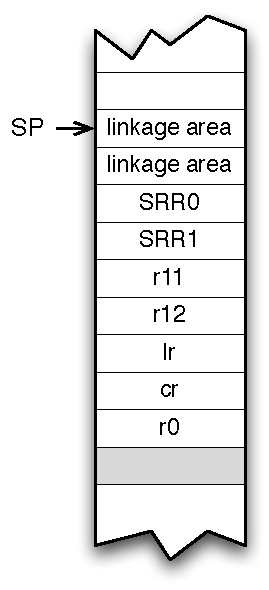
\includegraphics[scale=.6]{pictures/TFStack2} 
\end{minipage}
\begin{minipage}{0.5\textwidth}
  \caption{Process stack mapping when the trusted function starts its execution.}\label{fig:tfstackmapping2}
\end{minipage}
\end{figure}

\subsection{The ExitTrustedFunction service}\label{sec:exittfppc}

When a trusted function finishes, the context of the \api{CallTrustedFunction} must be restored to return to the caller. \api{ExitTrustedFunction} should not be called explicitly because its address has been set as the return address of the trusted function by \cfunction{tpl_call_trusted_function_service}. Calling \api{ExitTrustedFunction} explicitly would result in an undefined behavior or in the crash of the calling process but see below. The mapping of the process stack at start of \cfunction{tpl_exit_trusted_function_service} is shown in figure \ref{fig:ETFstack1}.

\begin{figure}[htbp] %  figure placement: here, top, bottom, or page
\begin{minipage}{0.4\textwidth}
    \centering
  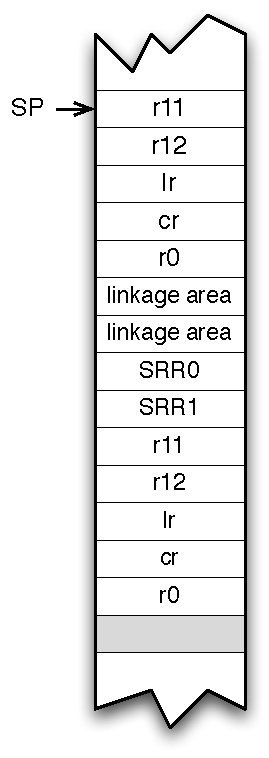
\includegraphics[scale=.6]{pictures/ETFStack1} 
\end{minipage}
\begin{minipage}{0.6\textwidth}
  \caption{Process stack mapping when the \cfunction{tpl_exit_trusted_function_service} function starts its execution.}\label{fig:ETFstack1}
\end{minipage}
\end{figure}

First, \cfunction{tpl_exit_trusted_function_service} decrements the trusted counter of the calling process. A particular attention must be given to this point because by building a fake stack frame and calling Explicitly \api{ExitTrustedFunction} to underflow this counter, a process could get a full access to the memory. So the counter is tested before to avoid to go under 0.

\begin{lstlisting}[language=C]
  lwz   r11,KS_KERN_PTR(r1)   /* get the ptr to tpl_kern */
  lwz   r11,12(r11)           /* get the ptr to the runnning process desc */
  lwz   r12,4(r11)            /* get trusted_count member */
  /*
   * Warning, the trusted counter has to be check (compared to 0) to
   * avoid to decrement it if it is already 0. Without that a process
   * could build an had-hoc stack an call explicitly ExitTrustedFunction
   * to get access to all the memory.
   */
  cmpwi r12,0                 /* check it is not already at 0 */
  beq   cracker_in_action     /* uh uh */
  subi  r12,r12,1             /* decrement it */
  stw   r12,4(r11)            /* put it back in the process desc */
\end{lstlisting}

\cfunction{tpl_exit_trusted_function_service} has to remove from the process stack the frame that was built by \cfunction{tpl_call_trusted_function_service}, restore \reg{SRR0} and \reg{SRR1} before returning to the dispatch layer.

\begin{lstlisting}[language=C]
cracker_in_action:
  
  /*
   * get the process stack pointer
   */
  lwz   r11,KS_SP(r1)
  
  /*
   * get back the SRR0 and SRR1
   */
  lwz   r12,PS_SRR0_OUT(r11)
  stw   r12,KS_SRR0(r1)
  lwz   r12,PS_SRR1_OUT(r11)
  stw   r12,KS_SRR1(r1)
  
  /*
   * free the process stack and update it in the kernel stack
   */
  addi  r11,r11,PS_TRUSTED_FOOTPRINT_OUT
  stw   r11,KS_SP(r1)
  
  /*
   * that's all
   */
  blr
\end{lstlisting}

\subsection{The MPC5510 Memory Protection Unit}

The access control rights of the memory region descriptor rules the access of 5 bus masters (labeled from 4 to 0). Unused bus masters are set to the same access right for all the regions. Bus master 4 is used for factory testing only, so the access rights should be set to no access. Bus master 3 is the Flexray controller. Since it is not used in the current version of Trampoline, it is set to no access to. Bus master 2 is the DMA controller. For the same reason it is set to no access. Bus master 1 is the Z0 core. Again it is set to no access.

The access control rights register has the following bit usage:

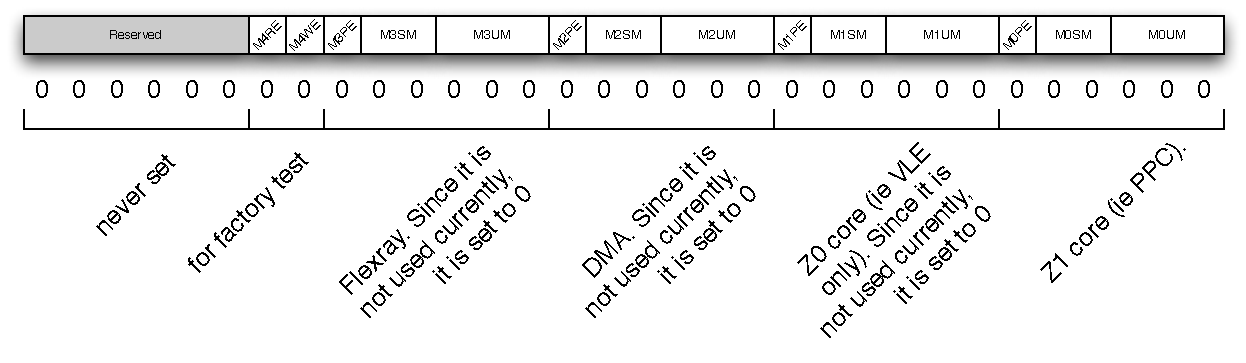
\includegraphics[width=\textwidth]{pictures/MPUacr.pdf} 

Bus master 4 is a special case. The 2 bits have the following meaning:

\rowcolors{1}{white}{light-gray}
\begin{longtableii}{p{0.4in}|p{4.8in}}{}{Bit}{Meaning}
  \lineii{M4RE}
  {If set to 1, bus master 4 may \strong{read} memory in the region. If 0, no read is allowed}
  \lineii{M4WE}
  {If set to 1, bus master 4 may \strong{write} memory in the region. If 0, no write is allowed}
\end{longtableii}

So in our case, these bits are set to 0.

Of course, other bus masters have more sophisticated access right:

\rowcolors{1}{white}{light-gray}
\begin{longtableii}{p{0.4in}|p{4.8in}}{}{Bit}{Meaning}
  \lineii{MxPE}
  {The PID Enable bit. Set to 0 in our case}
  \lineii{MxSM}
  {These 2 bits rules the supervisor mode access control with the following meaning: $00=rwx$, $01=rx$, $10=rw$, $11=$ \textit{same as defined by MxUM}. In our case, it is set to $00$ for code and constants and to $11$ for data.}
  \lineii{MxUM}
  {These 2 bits rules the user mode access control. The first bit means $r$, the second one $w$ and the third one $x$.}
\end{longtableii}

Trampoline uses 4 descriptors:

\rowcolors{1}{white}{light-gray}
\begin{longtableiii}{p{0.8in}|p{2in}|p{2.3in}}{}{Descriptor}{Usage}{MxUM value}
  \lineiii{MPU\_RGD0}
  {Constants and program\footnote{This region is set to the whole addressing space. This is not definitive and should be improved because reading a peripheral control register should be protected. So an additional descriptor has to be used to allow the kernel (supervisor mode) a complete access on all the memory space and no access at all for applications (user mode).}.}
  {$rwx=00$ for supervisor mode, $rx=101$ for user mode.}
  \lineiii{MPU\_RGD1}
  {Private variables of the process.}
  {$rw=110$ for supervisor and user mode.}
  \lineiii{MPU\_RGD2}
  {Stack of the process.}
  {$rw=110$ for supervisor and user mode.}
  \lineiii{MPU\_RGD3}
  {Variables of the OS Application if OS Applications are used.}
  {$rw=110$ for supervisor and user mode.}
\end{longtableiii}

So values of access control bits should be:

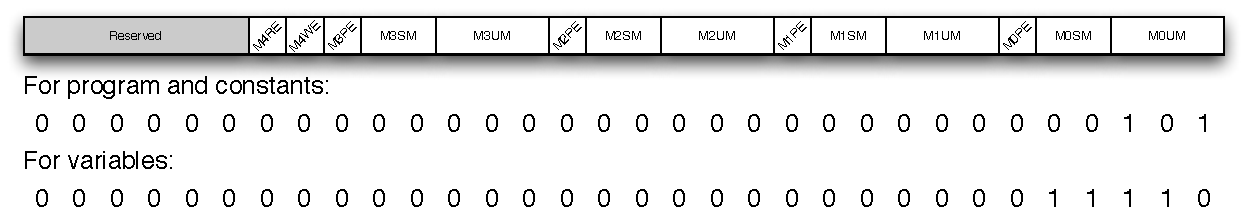
\includegraphics[width=\textwidth]{pictures/MPUprog.pdf} 

So in hexa:

\rowcolors{1}{white}{light-gray}
\begin{longtableii}{l|l}{}{Kind}{Value}
  \lineii{Program region access}
  {$0x00000005$}
  \lineii{Variable region access}
  {$0x0000001E$}
\end{longtableii}

\subsubsection{What happen in case of memory protection violation ?}

Two exception handler are used to handle a memory protection violation, one for data access, one for code access.

The Data Storage exception is tied to the IVOR~2 vector (VPR offset = 0x020), see page 8-2 of the {\em MPC5510 Microcontroller Family Reference Manual}.

The Instruction Storage exception is tied to the IVOR~3 vector (VPR offset = 0x030), see page 8-2 of the {\em MPC5510 Microcontroller Family Reference Manual}.

However, it appears one of these exceptions is raised when the processor is in user mode. The behavior is different in supervisor mode {\em to be completed}.



\part{The Goil system generator}

%!TEX root = ./trampoline.tex

\chapter{The Goil templates}

Goil includes a template interpreter which is used for file generation. Goil generates the structures needed by trampoline to compile the application and may generate other files like a memory mapping file \file{MemMap.h}, the compiler abstraction files, \file{Compiler.h} and \file{Compiler\_cfg.h} and a linker script depending on which attributes you set in the OIL file. 

A template is a file which is located in the default template directory (set with the environment variable \envvar{GOIL\_TEMPLATES} or with the \longprogramopt{templates} option on the command line) or in the directory of your project. Goil starts by looking for a template in the directory of your project, then, if the template is not found, in the default templates directory.

Four sets of templates are used:
\begin{itemize}
\item code generation templates that are located in the \file{code} subdirectory of the template directory;
\item build system templates that are located in the \file{build} subdirectory;
\item compiler dependent stuff in the \file{compiler} subdirectory and
\item linker script templates in the \file{linker} subdirectory.
\end{itemize}

Templates are written using a simple language which allow to access the application configuration data and to mix them with text to produce files.

Files are produced by a template program located in the \file{root.goilTemplate} file which is as the root of the template directory. By default the following files are produced:
\begin{itemize}
\item \file{tpl\_app\_config.c} by using the \file{tpl\_app\_config.c.goilTemplate} file
\item \file{tpl\_app\_config.h} by using the \file{tpl\_app\_config.h.goilTemplate} file
\item \file{Makefile} (if option \programopt{g} or \longprogramopt{generate-makefile} is given) by using the \file{Makefile.goilTemplate} file
\item \file{script.ld} (if memory mapping is used and if the default name is not changed) by using the \file{script.goilTemplate} file
\item \file{MemMap.h} (if memory mapping is used) by using the \file{MemMap.h.goilTemplate} file
\item \file{Compiler.h} (if memory mapping is used) by using the \file{Compiler.h.goilTemplate} file
\item \file{Compiler\_Cfg.h} (if memory mapping is used) by using the\\\file{Compiler\_Cfg.h.goilTemplate} file
\end{itemize}

\section{The configuration data}

The configuration data are computed by Goil from the OIL source files, from the options on the command line and from the \file{target.cfg} file. They are available as a set of predefined boolean, string, integer or list variables. All these variables are in capital letters.

\warning{Some configuration data are not listed here because they are dependent on the target. For instance, the \member{STACKSIZE} data may be an attribute of each item of a \var{TASKS} list for ppc target but are missing for the c166 target.}

\subsection{The \var{PROCESSES}, \var{TASKS}, \var{BASICTASKS}, \var{EXTENDEDTASKS}, \var{ISRS1} and \var{ISRS2} lists}

Theses variables are lists where informations about the processes\footnote{In Trampoline, a process is a task or an ISR category 2.} used in the application are stores:

\rowcolors{1}{white}{light-gray}
\begin{longtableii}{p{1.2in}|p{4in}}{var}{List}{Content}
  \lineii{PROCESSES}
  {the list of processes. The items are sorted in the following order: extended tasks, then basic tasks, then ISRs category 2.}
  \lineii{TASKS}
  {the list of tasks, basic and extended. The items are sorted in the following order: extended tasks, then basic tasks.}
  \lineii{BASICTASKS}
  {the list of basic tasks.}
  \lineii{EXTENDEDTASKS}
  {the list of extended tasks.}
  \lineii{ISRS1}
  {the list of ISR category 1.}
  \lineii{ISRS2}
  {the list of ISR category 2.}
\end{longtableii}

Each item of these lists has the following attributes:

\rowcolors{1}{white}{light-gray}
\begin{longtableiii}{p{1.6in}|l|p{3in}}{member}{Item}{Type}{Content}
  \lineiii{NAME}
  {string}
  {the name of the process.}
  \lineiii{PROCESSKIND}
  {string}
  {the kind of process: \stringlit{Task} or \stringlit{ISR}.}
  \lineiii{EXTENDEDTASK}
  {boolean}
  {true if the process is an extended task, false otherwise.}
  \lineiii{NONPREEMPTABLE}
  {boolean}
  {true if the process is a non-preemptable task, false otherwise.}
  \lineiii{PRIORITY}
  {integer}
  {the priority of the process.}
  \lineiii{ACTIVATION}
  {integer}
  {the number of activation of a task. 1 for and extended task or an ISR.}
  \lineiii{AUTOSTART}
  {boolean}
  {true if the process is an autostart task, false otherwise.}
  \lineiii{USEINTERNALRESOURCE}
  {boolean}
  {true if the process is a task that uses an internal resource, false otherwise.}
  \lineiii{INTERNALRESOURCE}
  {string}
  {the name of the internal resource if the process is a task that uses an internal resource, empty string otherwise.}
  \lineiii{RESOURCES}
  {list}
  {The resources used by the process. Each item has the following attribute: \member{NAME}}
\end{longtableiii}

\subsection{The \var{COUNTERS}, \var{HARDWARECOUNTERS} and \var{SOFTWARECOUNTERS} lists}

This list contains all the informations about the counters used in the application, including the \var{SystemCounter}.

\rowcolors{1}{white}{light-gray}
\begin{longtableii}{p{1.5in}|p{3.7in}}{var}{List}{Content}
  \lineii{COUNTERS}
  {the list of counters, both hardware and software as long as the \var{SystemCounter}}
  \lineii{HARDWARECOUNTERS}
  {the list of hardware counters including the \var{SystemCounter}.}
  \lineii{SOFTWARECOUNTERS}
  {the list of software counters.}
\end{longtableii}

Each item of this list has the following attributes:

\rowcolors{1}{white}{light-gray}
\begin{longtableiii}{p{1.6in}|l|p{3in}}{member}{Item}{Type}{Content}
  \lineiii{NAME}
  {string}
  {the name of the counter.}
  \lineiii{TYPE}
  {string}
  {the type of counter: {\small\stringlit{HARDWARE_COUNTER}} or {\small\stringlit{SOFTWARE_COUNTER}}.}
  \lineiii{MAXALLOWEDVALUE}
  {integer}
  {the maximum allowed value of the counter.}
  \lineiii{MINCYCLE}
  {integer}
  {the minimum cycle value of the counter.}
  \lineiii{TICKPERBASE}
  {integer}
  {the number of ticks needed to increment the counter.}
  \lineiii{SOURCE}
  {string}
  {the interrupt source name of the counter. This can be used to wrap interrupt vector to a counter incrementation function}
\end{longtableiii}

\subsection{The \var{EVENTS} list}

This list contains the informations about the events of the application. Each item has the following attributes:

\rowcolors{1}{white}{light-gray}
\begin{longtableiii}{p{1.6in}|l|p{3in}}{member}{Item}{Type}{Content}
  \lineiii{NAME}
  {string}
  {the name of the event.}
  \lineiii{MASK}
  {integer}
  {the mask of the event.}
\end{longtableiii}

\subsection{The \var{ALARMS} list}

This list contains the informations about the alarms of the application. Each item has the following attributes:

\rowcolors{1}{white}{light-gray}
\begin{longtableiii}{p{1.6in}|l|p{3in}}{member}{Item}{Type}{Content}
  \lineiii{NAME}
  {string}
  {the name of the alarm.}
  \lineiii{COUNTER}
  {string}
  {the name of the counter that drives the alarm.}
  \lineiii{ACTION}
  {string}
  {the action to be done when the alarm expire. It can take the following values: \stringlit{setEvent}, \stringlit{activateTask} and \stringlit{callback}. The last action is not available in Autosar mode.}
  \lineiii{TASK}
  {string}
  {the name of the task on which the action is performed. This attribute is defined for \stringlit{setEvent} and \stringlit{activateTask} actions only.}
  \lineiii{EVENT}
  {string}
  {the name of the event to set on the target task. This attribute is defined for \stringlit{setEvent} action only.}
  \lineiii{AUTOSTART}
  {boolean}
  {true if the alarm is autostart, false otherwise}
  \lineiii{ALARMTIME}
  {integer}
  {the alarm time of the alarm. This attribute is set if \member{AUTOSTART} is true}
  \lineiii{CYCLETIME}
  {integer}
  {the cycle time of the alarm. This attribute is set if \member{AUTOSTART} is true}
  \lineiii{APPMODE}
  {string}
  {the application mode in which the alarm is autostart. This attribute is set if \member{AUTOSTART} is true}
\end{longtableiii}

\subsection{The \var{REGULARRESOURCES} and \var{INTERNALRESOURCES} lists}

These lists contains the informations about the resources of the application.

\rowcolors{1}{white}{light-gray}
\begin{longtableii}{p{1.5in}|p{3.7in}}{var}{List}{Content}
  \lineii{REGULARRESOURCES}
  {the list of STANDARD and LINKED resources.}
  \lineii{INTERNALRESOURCES}
  {the list of INTERNAL resources.}
\end{longtableii}

Each item has the following attributes:

\rowcolors{1}{white}{light-gray}
\begin{longtableiii}{p{1.6in}|l|p{3in}}{member}{Item}{Type}{Content}
  \lineiii{NAME}
  {string}
  {the name of the resource.}
  \lineiii{PRIORITY}
  {integer}
  {the priority of the resource.}
  \lineiii{TASKUSAGE}
  {list}
  {the list of tasks that use the resource. Each item of this list has an attribute \member{NAME} which is the name of the task.}
  \lineiii{ISRUSAGE}
  {list}
  {the list of ISRs that use the resource. Each item of this list has an attribute \member{NAME} which is the name of the ISR.}
\end{longtableiii}

\subsection{The \var{MESSAGES}, \var{SENDMESSAGES} and \var{RECEIVEMESSAGES} lists}

These lists contain the informations about the messages of the application.

\rowcolors{1}{white}{light-gray}
\begin{longtableii}{p{1.5in}|p{3.7in}}{var}{List}{Content}
  \lineii{MESSAGES}
  {the list of messages, both send and receive message.}
  \lineii{SENDMESSAGES}
  {the list of send messages.}
  \lineii{RECEIVEMESSAGES}
  {the list of receive messages.}
\end{longtableii}

Each item has the following attributes

\rowcolors{1}{white}{light-gray}
\begin{longtableiii}{p{1.6in}|l|p{3in}}{member}{Item}{Type}{Content}
  \lineiii{NAME}
  {string}
  {the name of the message.}
  \lineiii{MESSAGEPROPERTY}
  {string}
  {the type of the message. It can be {\small\stringlit{RECEIVE\_ZERO\_INTERNAL}, \stringlit{RECEIVE\_UNQUEUED\_INTERNAL}, \stringlit{RECEIVE\_QUEUED\_INTERNAL}, \stringlit{SEND\_STATIC\_INTERNAL}, \stringlit{SEND\_ZERO\_INTERNAL} or \stringlit{RECEIVE\_ZERO\_SENDERS}}.}
  \lineiii{NEXT}
  {string}
  {the name of the next message in a receive message chain. This attribute is defined for receive messages only.}
  \lineiii{SOURCE}
  {string}
  {the name of the send message which is connected to the receive message. This attribute is defined for receive messages only.}
  \lineiii{CTYPE}
  {string}
  {the C language type of the message. This attribute is not defined for {\small\stringlit{RECEIVE\_ZERO\_INTERNAL}} and  {\small\stringlit{SEND\_ZERO\_INTERNAL}} messages.}
  \lineiii{INITIALVALUE}
  {string}
  {initial value of the receive message. This attribute is defined for {\small\stringlit{RECEIVE\_UNQUEUED\_INTERNAL}} and  {\small\stringlit{RECEIVE\_ZERO\_SENDERS}} messages only.}
  \lineiii{QUEUESIZE}
  {integer}
  {queue size of a receive queued message. This attribute is defined for {\small\stringlit{RECEIVE\_QUEUED\_INTERNAL}} messages only.}
  \lineiii{TARGET}
  {string}
  {target message of a send message. This is the first message in a receive message chain. This attribute is defined for {\small\stringlit{SEND\_STATIC\_INTERNAL}} and {\small\stringlit{SEND\_ZERO\_INTERNAL}} messages only.}
  \lineiii{FILTER}
  {string}
  {the kind of filter to apply. This attribute may take the following values: {\small\stringlit{ALWAYS}, \stringlit{NEVER}, \stringlit{MASKEDNEWEQUALSX}, \stringlit{MASKEDNEWDIFFERSX}, \stringlit{NEWISEQUAL}, \stringlit{NEWISDIFFERENT}, \stringlit{MASKEDNEWEQUALSMASKEDOLD}, \stringlit{MASKEDNEWDIFFERSMASKEDOLD}, \stringlit{NEWISWITHIN}, \stringlit{NEWISOUTSIDE}, \stringlit{NEWISGREATER}, \stringlit{NEWISLESSOREQUAL}, \stringlit{NEWISLESS}, \stringlit{NEWISGREATEROREQUAL}} or {\small\stringlit{ONEEVERYN}}.}
  \lineiii{MASK}
  {integer}
  {Mask of the filter when needed. This attribute is defined for {\small\stringlit{MASKEDNEWEQUALSX}, \stringlit{MASKEDNEWDIFFERSX}, \stringlit{MASKEDNEWEQUALSMASKEDOLD}} and {\small\stringlit{MASKEDNEWDIFFERSMASKEDOLD}} filters only.}
  \lineiii{X}
  {integer}
  {Value of the filter when needed. This attribute is defined for {\small\stringlit{MASKEDNEWEQUALSMASKEDOLD}} and {\small\stringlit{MASKEDNEWDIFFERSX}} filters only.}
  \lineiii{MIN}
  {integer}
  {Minimum value of the filter when needed. This attribute is defined for {\small\stringlit{NEWISWITHIN}} and {\small\stringlit{NEWISOUTSIDE}} filters only.}
  \lineiii{MAX}
  {integer}
  {Maximum value of the filter when needed. This attribute is defined for {\small\stringlit{NEWISWITHIN}} and {\small\stringlit{NEWISOUTSIDE}}}     
  \lineiii{PERIOD}
  {integer}
  {Period of the filter. This attribute is defined for {\small\stringlit{ONEEVERYN}} filter only.}
  \lineiii{OFFSET}
  {integer}
  {Offset of the filter. This attribute is defined for {\small\stringlit{ONEEVERYN}} filter only.}
  \lineiii{ACTION}
  {string}
  {the action (or notification) to be done when the message is delivered. It can take the following values: \stringlit{setEvent} or \stringlit{activateTask}.}
  \lineiii{TASK}
  {string}
  {the name of the task on which the notification is performed. This attribute is defined for \stringlit{setEvent} and \stringlit{activateTask} actions only.}
  \lineiii{EVENT}
  {string}
  {the name of the event to set on the target task. This attribute is defined for \stringlit{setEvent} notification only.}
\end{longtableiii}

\subsection{The \var{SCHEDULETABLES} list}

This list contains the informations about the schedule tables of the application.

\rowcolors{1}{white}{light-gray}
\begin{longtableiii}{p{1.6in}|l|p{3in}}{member}{Item}{Type}{Content}
  \lineiii{NAME}
  {string}
  {the name of the schedule table.}
  \lineiii{COUNTER}
  {string}
  {the name of the counter which drives the schedule table.}
  \lineiii{PERIODIC}
  {boolean}
  {true if the schedule table is a periodic one, false otherwise.}
  \lineiii{SYNCSTRATEGY}
  {string}
  {the synchronization strategy of the schedule table. This attribute may take the following values: {\small\stringlit{SCHEDTABLE_NO_SYNC}, \stringlit{SCHEDTABLE_IMPLICIT_SYNC}} or {\small\stringlit{SCHEDTABLE_EXPLICIT_SYNC}}.}
  \lineiii{PRECISION}
  {integer}
  {the precision of the synchronization. This attribute is define when \member{SYNCSTRATEGY} is {\small\stringlit{SCHEDTABLE_EXPLICIT_SYNC}}.}
  \lineiii{STATE}
  {string}
  {the state of the schedule table. This attribute may take the following values: {\small\stringlit{SCHEDULETABLE_STOPPED}, \stringlit{SCHEDULETABLE_AUTOSTART_SYNCHRON}, \stringlit{SCHEDULETABLE_AUTOSTART_RELATIVE}} or {\small\stringlit{SCHEDULETABLE_AUTOSTART_ABSOLUTE}}.}
  \lineiii{DATE}
  {integer}
  {the start date of the schedule table. This attribute has an actuel value when \member{STATE} is {\small\stringlit{SCHEDULETABLE_AUTOSTART_RELATIVE}} or {\small\stringlit{SCHEDULETABLE_AUTOSTART_ABSOLUTE}}, otherwise it is set to 0.}
  \lineiii{LENGTH}
  {integer}
  {The length of the schedule table.}
  \lineiii{EXPIRYPOINTS}
  {list}
  {The expiry points of the schedule table. See the following table for items attributes.}
\end{longtableiii}

Each item of the \member{EXPIRYPOINTS} list has the following attributes:

\rowcolors{1}{white}{light-gray}
\begin{longtableiii}{p{1.6in}|l|p{3in}}{member}{Item}{Type}{Content}
  \lineiii{ABSOLUTEOFFSET}
  {integer}
  {the absolute offset of the expiry points.}
  \lineiii{RELATIVEOFFSET}
  {integer}
  {the relative offset of the expiry points from the previous expiry point.}
  \lineiii{MAXRETARD}
  {integer}
  {maximum retard to keep the schedule table synchronous.}
  \lineiii{MAXADVANCE}
  {integer}
  {maximum advance to keep the schedule table synchronous.}
  \lineiii{ACTIONS}
  {list}
  {the actions to perform on the expiry point. See the following table for items attributes.}
\end{longtableiii}

Each item of the \member{ACTIONS} list has the following attributes:

\rowcolors{1}{white}{light-gray}
\begin{longtableiii}{p{1.6in}|l|p{3in}}{member}{Item}{Type}{Content}
  \lineiii{ACTION}
  {string}
  {the action to be done when the alarm expire. It can take the following values: \stringlit{setEvent}, \stringlit{activateTask}, \stringlit{incrementCounter} and \stringlit{finalizeScheduleTable}.}
  \lineiii{TASK}
  {string}
  {the name of the task on which the action is performed. This attribute is defined for \stringlit{setEvent} and \stringlit{activateTask} actions only.}
  \lineiii{EVENT}
  {string}
  {the name of the event to set on the target task. This attribute is defined for \stringlit{setEvent} action only.}
  \lineiii{TARGETCOUNTER}
  {string}
  {the name of the counter to increment. This attribute is defined for \stringlit{incrementCounter} action only.}
\end{longtableiii}

\subsection{The \var{OSAPPLICATIONS} list}

This list contains the informations about the OS Applications of the application.

\rowcolors{1}{white}{light-gray}
\begin{longtableiii}{p{2.1in}|l|p{2.5in}}{member}{Item}{Type}{Content}
  \lineiii{NAME}
  {string}
  {the name of the OS Application.}
  \lineiii{RESTART}
  {string}
  {the name of the restart task. This attribute is not defined is there is no restart task for the OS Application.}
  \lineiii{PROCESSACCESSVECTOR}
  {string}
  {access right for the processes}
  \lineiii{PROCESSACCESSITEMS}
  {string}
  {access right for the processes as bytes in a table}
  \lineiii{PROCESSACCESSNUM}
  {integer}
  {number of elements in the previous table}
  \lineiii{ALARMACCESSVECTOR}
  {string}
  {access right for the alarms}
  \lineiii{ALARMACCESSITEMS}
  {string}
  {access right for the alarms as bytes in a table}
  \lineiii{ALARMACCESSNUM}
  {integer}
  {number of elements in the previous table}
  \lineiii{RESOURCEACCESSVECTOR}
  {string}
  {access right for the resources}
  \lineiii{RESOURCEACCESSITEMS}
  {string}
  {access right for the resources as bytes in a table}
  \lineiii{RESOURCEACCESSNUM}
  {integer}
  {number of elements in the previous table}
  \lineiii{SCHEDULETABLEACCESSVECTOR}
  {string}
  {access right for the schedule tables}
  \lineiii{SCHEDULETABLEACCESSITEMS}
  {string}
  {access right for the schedule tables as bytes in a table}
  \lineiii{SCHEDULETABLEACCESSNUM}
  {integer}
  {number of elements in the previous table}
  \lineiii{COUNTERACCESSVECTOR}
  {string}
  {access right for the software counters}
  \lineiii{COUNTERACCESSITEMS}
  {string}
  {access right for the software counters as bytes in a table}
  \lineiii{COUNTERACCESSNUM}
  {integer}
  {number of elements in the previous table}
  \lineiii{PROCESSES}
  {list}
  {list of the processes that belong to the OS Application. Each item has an attribute \member{NAME} which is the name of the process.}
  \lineiii{HASSTARTUPHOOK}
  {boolean}
  {true if the OS Application has a startup hook.}
  \lineiii{HASSHUTDOWNHOOK}
  {boolean}
  {true if the OS Application has a shutdown hook.}
  \lineiii{TASKS}
  {list}
  {list of the tasks that belong to the OS Application. Each item has an attribute \member{NAME} which is the name of the task.}
  \lineiii{ISRS}
  {list}
  {list of the ISRs that belong to the OS Application. Each item has an attribute \member{NAME} which is the name of the ISR.}
  \lineiii{ALARMS}
  {list}
  {list of the alarms that belong to the OS Application. Each item has an attribute \member{NAME} which is the name of the alarm.}
  \lineiii{RESOURCES}
  {list}
  {list of the resources that belong to the OS Application. Each item has an attribute \member{NAME} which is the name of the resource.}
  \lineiii{REGULARRESOURCES}
  {list}
  {list of the standard or linked resources that belong to the OS Application. Each item has an attribute \member{NAME} which is the name of the resource.}
  \lineiii{INTERNALRESOURCES}
  {list}
  {list of the internal resources that belong to the OS Application. Each item has an attribute \member{NAME} which is the name of the resource.}
  \lineiii{SCHEDULETABLES}
  {list}
  {list of the schedule tables that belong to the OS Application. Each item has an attribute \member{NAME} which is the name of the schedule table.}
  \lineiii{COUNTERS}
  {list}
  {list of the counters that belong to the OS Application. Each item has an attribute \member{NAME} which is the name of the counter.}
  \lineiii{MESSAGES}
  {list}
  {list of the messages that belong to the OS Application. Each item has an attribute \member{NAME} which is the name of the messages.}
\end{longtableiii}

\subsection{The \var{TRUSTEDFUNCTIONS} list}

This list contains the informations about the trusted functions of the application. Each item contains one attribute only.

\rowcolors{1}{white}{light-gray}
\begin{longtableiii}{p{1.6in}|l|p{3in}}{member}{Item}{Type}{Content}
  \lineiii{NAME}
  {string}
  {the name of the trusted function.}
\end{longtableiii}

\subsection{The \var{READLIST} list}

This list contains the informations about the ready list. Items are sorted by priority from 0 to the maximum computed priority. The only attribute of each item is the size of the queue.

\rowcolors{1}{white}{light-gray}
\begin{longtableiii}{p{1.6in}|l|p{3in}}{member}{Item}{Type}{Content}
  \lineiii{SIZE}
  {integer}
  {the size of the queue for the corresponding priority.}
\end{longtableiii}

\subsection{The \var{SOURCEFILES}, \var{CFLAGS}, \var{CPPFLAGS}, \var{ASFLAGS}, \var{LDFLAGS} and \var{TRAMPOLINESOURCEFILES} lists}

The \var{SOURCEFILES} list contains the source files as found in attributes \member{APP\_SRC} of the OS object in the OIL file.

\rowcolors{1}{white}{light-gray}
\begin{longtableiii}{p{1.6in}|l|p{3in}}{member}{Item}{Type}{Content}
  \lineiii{FILE}
  {string}
  {the source file name.}
\end{longtableiii}

The \var{CFLAGS} list contains the flags for the C compiler as found in attributes \member{CFLAGS} of the OS object in the OIL file.

\rowcolors{1}{white}{light-gray}
\begin{longtableiii}{p{1.6in}|l|p{3in}}{member}{Item}{Type}{Content}
  \lineiii{CFLAG}
  {string}
  {the C compiler flag.}
\end{longtableiii}

The \var{CPPFLAGS} list contains the flags for the C++ compiler as found in attributes \member{CPPFLAGS} of the OS object in the OIL file.

\rowcolors{1}{white}{light-gray}
\begin{longtableiii}{p{1.6in}|l|p{3in}}{member}{Item}{Type}{Content}
  \lineiii{CPPFLAG}
  {string}
  {the C++ compiler flag.}
\end{longtableiii}

The \var{ASFLAGS} list contains the flags for the assembler as found in attributes \member{ASFLAGS} of the OS object in the OIL file.

\rowcolors{1}{white}{light-gray}
\begin{longtableiii}{p{1.6in}|l|p{3in}}{member}{Item}{Type}{Content}
  \lineiii{ASFLAG}
  {string}
  {the assembler flag.}
\end{longtableiii}

The \var{LDFLAGS} list contains the flags for the linker as found in attributes \member{LDFLAGS} of the OS object in the OIL file.

\rowcolors{1}{white}{light-gray}
\begin{longtableiii}{p{1.6in}|l|p{3in}}{member}{Item}{Type}{Content}
  \lineiii{LDFLAG}
  {string}
  {the linker flag.}
\end{longtableiii}

The \var{TRAMPOLINESOURCEFILES} list contains the trampoline source files used by the application.

\rowcolors{1}{white}{light-gray}
\begin{longtableiii}{p{1.6in}|l|p{3in}}{member}{Item}{Type}{Content}
  \lineiii{DIRECTORY}
  {string}
  {the directory of the source file relative to the Trampoline root directory (\file{os}, \file{com} or \file{autosar}).}
  \lineiii{FILE}
  {string}
  {the source file name.}
\end{longtableiii}


\subsection{The \var{INTERRUPTSOURCES} list}

This list is extracted from the \file{target.cfg} file. Each item has the following attribute:

\rowcolors{1}{white}{light-gray}
\begin{longtableiii}{p{1.6in}|l|p{3in}}{member}{Item}{Type}{Content}
  \lineiii{NAME}
  {string}
  {the name of the interrupt source. This is one of the name used in the OIL file as value for the \member{SOURCE} attribute}
  \lineiii{NUMBER}
  {string}
  {the id of the interrupt source.}
\end{longtableiii}



\subsection{Scalar data}

The following scalar data are defined:

\rowcolors{1}{white}{light-gray}
\begin{longtableiii}{p{1.6in}|l|p{3in}}{member}{Data}{Type}{Content}
\lineiii{APPNAME}
{string}
{name of executable as given in the \member{APP\_NAME} attribute in the OS object} 
\lineiii{ARCH}
{string}
{name of the architecture. This is the first item in the target.} 
\lineiii{ASSEMBLEREXE}
{string}
{name of the assembler executable used. This is the \member{ASSEMBLER} attribute in the OS object. It is set to {\em as} by default. It is used for build dependent templates.} 
\lineiii{ASSEMBLER}
{string}
{name of the assembler used. This is the \member{ASSEMBLER} attribute in the \member{MEMMAP} attribute of the OS object. It is used for assembler dependent templates.} 
\lineiii{AUTOSAR}
{boolean}
{true if Trampoline is compiled with the Autosar extension.} 
\lineiii{BOARD}
{string}
{name of the board. This is the third item (if any) in the target.} 
\lineiii{CHIP}
{string}
{name of the chip. This is the second item (if any) in the target.} 
\lineiii{COMPILEREXE}
{string}
{name of the compiler executable used. This is the \member{COMPILER} attribute in the OS object. It is set to {\em gcc} by default. It is used for build dependent templates. Do not confuse with the \member{COMPILER} data.} 
\lineiii{COMPILER}
{string}
{name of the compiler used. This is the \member{COMPILER} attribute in the \member{MEMMAP} attribute of the OS object. It is used for compiler dependent templates.} 
\lineiii{CPUNAME}
{string}
{name given to the OIL CPU object} 
\lineiii{EXTENDED}
{boolean}
{true if Trampoline is compiled in extended error handling mode.} 
\lineiii{FILENAME}
{string}
{the name of the file which will be written as the result of the computation of the current template.} 
\lineiii{FILEPATH}
{string}
{the full absolute path of the file which will be written as the result of the computation of the current template.} 
\lineiii{NATIVEFILEPATH}
{string}
{the full absolute path of the file which will be written as the result of the computation of the current template in native OS format.} 
\lineiii{ITSOURCESLENGTH}
{integer}
{number of interrupt sources as defined in the \file{target.cfg} file.} 
\lineiii{LINKEREXE}
{string}
{name of the linker executable used. This is the \member{LINKER} attribute in the OS object. It is set to {\em gcc} by default. It is used for build dependent templates. Do not confuse with the \member{LINKER} data.} 
\lineiii{LINKER}
{string}
{name of the linker used. This is the \member{LINKER} attribute in the \member{MEMMAP} attribute of the OS object. It is used for linker dependent templates.} 
\lineiii{LINKSCRIPT}
{string}
{name of the link script file as given in the \member{MEMMAP} attribute of the OS object.} 
\lineiii{MAXTASKPRIORITY}
{integer}
{the highest computed priority among the tasks.} 
\lineiii{OILFILENAME}
{string}
{name of the root OIL source file} 
\lineiii{PROJECT}
{string}
{name of the project. The name of the project is the \programopt{p} (or \longprogramopt{project}) value if it is set or the name of the oil file without the extension.} 
\lineiii{SCALABILITYCLASS}
{integer}
{the Autosar scalability class used by the application. If Autosar is not enabled, \member{SCALABILITYCLASS} is set to 0.} 
\lineiii{TARGET}
{string}
{name of the target. This is the \programopt{t} (or \longprogramopt{target}) option value of goil.} 
\lineiii{TEMPLATEPATH}
{string}
{path to the template root directory. This is the \longprogramopt{templates} option value of goil or the value of the \envvar{GOIL\_TEMPLATES} environment variable.} 
\lineiii{TIMESTAMP}
{string}
{current date} 
\lineiii{TRAMPOLINEPATH}
{string}
{path to the trampoline root directory. This is the \member{TRAMPOLINE\_BASE\_PATH} attribute of the OS object. It defaults to ``..".} 
\lineiii{USECOMPILERSETTINGS}
{boolean}
{true if memory mapping is enabled (Goil generates the \file{Compiler.h} and \file{Compiler_Cfg.h} files and Trampoline includes them).} 
\lineiii{USEBUILDFILE}
{boolean}
{true if a build file is used for the project ie option \programopt{g} or \longprogramopt{generate-makefile} is given.} 
\lineiii{USECOM}
{boolean}
{true if the application uses OSEK COM.} 
\lineiii{USEERRORHOOK}
{boolean}
{true if Trampoline uses the Error Hook.} 
\lineiii{USEGETSERVICEID}
{boolean}
{true if Trampoline uses the service ids access macros.} 
\lineiii{USEINTERRUPTTABLE}
{boolean}
{true if the wrapping of interrupt vector to glue functions used to increment a counter or to activate an ISR2 (for instance) should be generated. The actual code generation is up to the port.} 
\lineiii{USELOGFILE}
{boolean}
{true if goil generates a log file, ie option \programopt{l} or \longprogramopt{logfile} is given.}
\lineiii{USEMEMORYMAPPING}
{boolean}
{true if memory mapping is enabled (Goil generates the \file{MemMap.h} file and Trampoline includes it).} 
\lineiii{USEMEMORYPROTECTION}
{boolean}
{true if Trampoline uses the Memory Protection.} 
\lineiii{USEOSAPPLICATION}
{boolean}
{true if Trampoline uses OS Applications.} 
\lineiii{USEPARAMETERACCESS}
{boolean}
{true if Trampoline uses the parmaters access macros.} 
\lineiii{USEPOSTTASKHOOK}
{boolean}
{true if Trampoline uses the Post-Task Hook.} 
\lineiii{USEPRETASKHOOK}
{boolean}
{true if Trampoline uses the Pre-Task Hook.} 
\lineiii{USEPROTECTIONHOOK}
{boolean}
{true if Trampoline uses the Protection Hook.} 
\lineiii{USERESSCHEDULER}
{boolean}
{true if Trampoline uses the RES_SCHEDULER resource.} 
\lineiii{USESHUTDOWNHOOK}
{boolean}
{true if Trampoline uses the Shutdown Hook.} 
\lineiii{USESTACKMONITORING}
{boolean}
{true if Trampoline uses the Stack Monitoring.} 
\lineiii{USESTARTUPHOOK}
{boolean}
{true if Trampoline uses the Startup Hook.} 
\lineiii{USESYSTEMCALL}
{boolean}
{true if services are called using a System Call (i.e. a software interrupt).} 
\lineiii{USETIMINGPROTECTION}
{boolean}
{true if Trampoline uses Timing Protection.} 
\lineiii{USETRACE}
{boolean}
{true if tracing is enabled.} 

\end{longtableiii}

\section{The Goil template language (or GTL)}

A template is a text file with file extension \file{.goilTemplate}. This kind of file mixes literal text with an embedded program. Some instructions (see section \ref{outputInstruction}) in the embedded program outputs text as a result of the program execution and this text is put in place of the instructions. The resulting file is then stored.

The template interpreter starts in literal text mode. Switching from literal text mode to program mode and back to text mode is done when a \character{\%} is encountered. A literal \character{\%} and a literal \character{\textbackslash} may be used by escaping them with a \character{\textbackslash}.

\section{GTL types}

GTL supports 4 types: \strong{string}, \strong{integer}, \strong{boolean} and \strong{list}. These types have readers %\footnote{All the readers available in the corresponding Galgas types are available}
to get informations about a variable. A reader is invoke with the following syntax:

\begin{lstlisting}
[expression reader]
\end{lstlisting}

\subsection{string readers}

The following readers are available for string variables:

\rowcolors{1}{white}{light-gray}
\begin{longtableiii}{p{2.2in}|l|p{2.4in}}{strong}{Item}{Type}{Meaning}
  \lineiii{HTMLRepresentation}
  {string}
  {this reader returns a representation of the string suitable for an HTML encoded representation. \character{\&} is encoded by \&amp; , \character{"} by \&quot; , \character{<} by \&lt; and \character{>} by \&gt; .}
  \lineiii{identifierRepresentation}
  {string}
  {this reader returns an unique representation of the string conforming to a C identifier. Any Unicode character that is not a latin letter is transformed into its hexadecimal code point value, enclosed by \character{_} characters. This representation is unique: two different strings are transformed into different C identifiers. For example: value3 is transformed to value\_33\_; += is transformed to \_2B\_\_3D;
An\_Identifier is transformed to An\_5F\_Identifier.}
  \lineiii{lowercaseString}
  {string}
  {this reader returns lowercased representation of the string.}
  \lineiii{length}
  {integer}
  {this reader returns the number of characters in the string}
  \lineiii{stringByCapitalizingFirstCharacter}
  {string}
  {if the string is empty, this reader returns the empty string; otherwise, it returns the string, the first character being replaced with the corresponding upper case character.}
  \lineiii{uppercaseString}
  {string}
  {this reader returns uppercased representation of the receiver}
\end{longtableiii}

\subsection{boolean readers}

The following readers are available for boolean variables:

\rowcolors{1}{white}{light-gray}
\begin{longtableiii}{p{2.2in}|l|p{2.4in}}{strong}{Item}{Type}{Meaning}
  \lineiii{trueOrFalse}
  {string}
  {this reader returns \stringlit{true} or \stringlit{false} according to the boolean value}
  \lineiii{yesOrNo}
  {string}
  {this reader returns \stringlit{yes} or \stringlit{no} according to the boolean value}
  \lineiii{unsigned}
  {integer}
  {this reader returns 0 or 1 according to the boolean value}
\end{longtableiii}

\subsection{integer readers}

The following readers are available for integer variables:

\rowcolors{1}{white}{light-gray}
\begin{longtableiii}{p{2.2in}|l|p{2.4in}}{strong}{Item}{Type}{Meaning}
  \lineiii{string}
  {string}
  {This reader returns the integer value as a character string.}
  \lineiii{hexString}
  {string}
  {this reader returns an hexadecimal string representation of the integer value.}
\end{longtableiii}

\subsection{list readers}

The following reader is available for list variables:

\rowcolors{1}{white}{light-gray}
\begin{longtableiii}{p{2.2in}|l|p{2.4in}}{strong}{Item}{Type}{Meaning}
  \lineiii{length}
  {integer}
  {this reader returns the number of objects currently in the list.}
\end{longtableiii}

\section{GTL operators}

\subsection{Unary operators}

\rowcolors{1}{white}{light-gray}
\begin{longtableiv}{c|l|l|p{2.4in}}{}{Operator}{Operand Type}{Result Type}{Meaning}
  \lineiv{+}
  {integer}
  {integer}
  {no operation.}
  \lineiv{$\sim$}
  {integer}
  {integer}
  {bitwise not.}
  \lineiv{not}
  {boolean}
  {boolean}
  {boolean not.}
  \lineiv{exists}
  {{\em any variable}}
  {boolean}
  {true if the variable is defined, false otherwise. But see below}
\end{longtableiv}

A second form of \strong{exists} is:
 
\begin{lstlisting}
exists var default (expression)
\end{lstlisting}

\var{var} and {\em expression} should have the same type. If \var{var} exists, the returned value is the content of \var{var}. If it does not exist, {\em expression} is returned.


\subsection{Binary operators}

\rowcolors{1}{white}{light-gray}
\begin{longtableiv}{c|l|l|p{2.27in}}{}{Operator}{Operands Type}{Result Type}{Meaning}
  \lineiv{+}
  {integer}
  {integer}
  {add.}
  \lineiv{-}
  {integer}
  {integer}
  {substract.}
  \lineiv{*}
  {integer}
  {integer}
  {multiply.}
  \lineiv{/}
  {integer}
  {integer}
  {divide.}
  \lineiv{\&}
  {integer}
  {integer}
  {Bitwise and.}
  \lineiv{\&}
  {boolean}
  {boolean}
  {boolean and.}
  \lineiv{$\mid$}
  {integer}
  {integer}
  {Bitwise or.}
  \lineiv{$\mid$}
  {boolean}
  {boolean}
  {boolean or.}
  \lineiv{$\wedge$}
  {integer}
  {integer}
  {Bitwise xor.}
  \lineiv{$\wedge$}
  {boolean}
  {boolean}
  {boolean xor.}
  \lineiv{.}
  {string}
  {string}
  {string concatenation.}
  \lineiv{$<<$}
  {integer}
  {integer}
  {shift left.}
  \lineiv{$>>$}
  {integer}
  {integer}
  {shift right.}
  \lineiv{!=}
  {{\em any}}
  {boolean}
  {comparison (different).}
  \lineiv{==}
  {{\em any}}
  {boolean}
  {comparison (equal).}
  \lineiv{$<$}
  {integer {\em or} boolean}
  {boolean}
  {comparison (lower than).}
  \lineiv{$<=$}
  {integer {\em or} boolean}
  {boolean}
  {comparison (lower or equal).}
  \lineiv{$>$}
  {integer {\em or} boolean}
  {boolean}
  {comparison (greater).}
  \lineiv{$>=$}
  {integer {\em or} boolean}
  {boolean}
  {comparison (greater or equal).}
\end{longtableiv}

\subsection{Constants}

\rowcolors{1}{white}{light-gray}
\begin{longtableiii}{p{2.2in}|l|p{2.4in}}{strong}{Constant}{Type}{Meaning}
  \lineiii{emptyList}
  {list}
  {this constant is an empty list}
  \lineiii{true}
  {boolean}
  {true boolean}
  \lineiii{false}
  {boolean}
  {false boolean}
  \lineiii{yes}
  {boolean}
  {true boolean}
  \lineiii{no}
  {boolean}
  {false boolean}
\end{longtableiii}

\section{GTL instructions}

\subsection{The {\em let} instruction}

Data assignment instruction. The general form is:

\begin{lstlisting}
let var := expression
\end{lstlisting}

A second form allows to add a string to a list (only, this should be extended in the future)

\begin{lstlisting}
let var += expression
\end{lstlisting}

\var{var} is a list and {\em expression} is a string.

The scope of a variable depends on the location where the variable is assigned the first time. For instance, in the following code:

\begin{lstlisting}
let a := 1
foreach TASKS do
  let b := INDEX
  let a := INDEX
end foreach
!a !b
\end{lstlisting}

Because a is assigned outside the {\bf foreach} loop, it contains the value of the last INDEX after the \strong{foreach}. Because b is assigned inside the \strong{foreach} loop, it does not exist after the loop anymore and \strong{!b} will trigger and error.


\subsection{The {\em if} instruction}

Conditional execution. The forms are:

\begin{lstlisting}
if expression then ... end if
if expression then ... else ... end if
if expression then ... elsif expression then ... end if
if expression then ... elsif expression then ... else ... end if
\end{lstlisting}    

The {\em expression} must be boolean. In the following example, the blue text (within the \%) is produced only if the USECOM boolean variable is true:

\begin{lstlisting}
if USECOM then %
#include "tpl_com.h" %
end if
\end{lstlisting}

\subsection{The {\em foreach} instruction}

This instruction iterates on the elements of a list. Each element may have many attributes that are available as variables within the {\bf do} section of the foreach loop. The simplest form is the following one

\begin{lstlisting}
foreach expression do ... end foreach
\end{lstlisting}

In the following example, for each element in the ALARMS list, the text between the {\bf do} and the {\bf end foreach} is produced with the NAME attribute of the current element of the ALARMS list inserted at the specified location. INDEX is not an attribute of the current element. It is generated for each element and ranges from 0 to the number of elements in the list minus 1.
\begin{lstlisting}
foreach ALARMS do
%
/* Alarm % !NAME % identifier */
#define % !NAME %_id % !INDEX %
CONST(AlarmType, AUTOMATIC) % !NAME % = % !NAME %_id;
%
end foreach
\end{lstlisting}

A more general form of the {\tt foreach} instruction is:

\begin{lstlisting}
foreach expression prefixedby string
  before ...
  do ...
  between ...
  after ...
end foreach
\end{lstlisting}

{\bf prefixedby} is optional and allows to prefix the attribute names by {\em string}. If the list is not empty, the {\bf before} section are executed once before the first execution of the {\bf do} section. The {\bf between} section is executed between the execution of the {\bf do} section.  If the list is not empty, the {\bf after} section is executed once after the last execution of the {\bf do} section.

In the following example, a table of pointers to alarm descriptors is generated:

\begin{lstlisting}
foreach ALARMS
  before %
tpl_time_obj *tpl_alarm_table[ALARM_COUNT] = {
%
  do %  &% !NAME %_alarm_desc%
  between %,
%
  after %
};
%
end foreach
\end{lstlisting}

\subsection{The {\em for} instruction}

The {\bf for} instruction iterates along a literal list of elements.

\begin{lstlisting}
for var in expression, ... , expression do
  ...
end for
\end{lstlisting}

At each iteration, {\em var} gets the value of the current {\em expression}. As in the {\bf foreach} instruction, INDEX is generated and ranges from 0 to the number of elements in the list minus 1.

\subsection{The {\em loop} instruction}

The {\bf loop} instruction is the classical integer loop. Its simplest form is:

\begin{lstlisting}
loop var from expression to expression do
  ...
end loop
\end{lstlisting}

Like in the foreach instruction, {\bf before},  {\bf between} and  {\bf after} sections may be used:

\begin{lstlisting}
loop var from expression to expression
  before ...
  do ...
  between ...
  after ...
end loop
\end{lstlisting}


\subsection{The {\em !} instruction}
\label{outputInstruction}

{\bf !} emits an expression. The form is:

\begin{lstlisting}
! expression
\end{lstlisting}

\subsection{The {\em ?} instruction}

{\bf ?} stores in a variable a number of spaces equal to the current column in the output. The form is:

\begin{lstlisting}
? var
\end{lstlisting}

\subsection{The {\em template} instruction}

The {\bf template} instruction includes the output of another template in the output of the current template. Its simplest form is the following one:

\begin{lstlisting}
template template_file_name
\end{lstlisting}

If the file {\em template\_file\_name}.goilTemplate does not exist, an error occurs. To include the output of a template without generating an error, use the following form:

\begin{lstlisting}
template if exists template_file_name
\end{lstlisting}

A third form allows to execute instructions when the included template file is not found:

\begin{lstlisting}
template if exists template_file_name or ... end template
\end{lstlisting}

At last, it is possible to search templates in a hierarchy (code, linker, compiler, build) different from the current one. For instance to include a template located in the linker hierarchy, use one of the following forms:

\begin{lstlisting}
template template_file_name in hierarchy
template if exists template_file_name in hierarchy
template if exists template_file_name in hierarchy or ... end template
\end{lstlisting}


In all cases, the included template inherits from the current variables table but works on its own local copy.

\subsection{The {\em write} instruction}

The write instruction defines a block where the template processing output is captured to be written to a file. The general form is:

\begin{lstlisting}
write to expression :
  ...
end write
\end{lstlisting}

Where {\em expression} is a string expression.

In the following example, the result of the \file{script} template is written to the link script file.

\begin{lstlisting}
if exists LINKER then
  write to PROJECT."/".LINKSCRIPT:
    template script in linker
  end write
end if
\end{lstlisting}


\subsection{The {\em error} and {\em warning} instructions}

It can be useful to generate an error or a warning if a data is not defined or if it looks strange. For instance if a target needs a \member{STACKSIZE} for a task or if the \member{STACKSIZE} is too large for a 16bit target. \strong{error} and \strong{warning} have 2 forms:

\begin{lstlisting}
error var expression
warning var expression
\end{lstlisting}

and

\begin{lstlisting}
error here expression
warning here expression
\end{lstlisting}

{\em expression} must be of type string. In the first form, \var{var} is a configuration data. The file location of this configuration may be a location in the OIL file or in the template file if the variable was assigned in the template. In the second form, \strong{here} means the current location in the template file.

In the following example an error is generated for each task with not \member{STACKSIZE} attribute in the OIL file:

\begin{lstlisting}
foreach TASKS do
  if not exists STACKSIZE then
    error NAME "STACKSIZE of Task " . NAME . " is not defined"
  end if
end foreach
\end{lstlisting}

In this second example, an error is generated if a template is not found:

\begin{lstlisting}
template if exists interrupt_wrapping or
  error here "interrupt_wrapping.goilTemplate not found"
end template
\end{lstlisting}

\section{Examples}

Here are examples of code generation using GTL.

\subsection{Computing the list of process ids}

\begin{lstlisting}
foreach PROCESSES do
  if PROCESSKIND == "Task" then
%
/* Task % !NAME % identifier */
#define % !NAME %_id % !INDEX %
CONST(TaskType, AUTOMATIC) % !NAME % = % !NAME %_id;
%
  else
%
/* ISR % !NAME % identifier */
#define % !NAME %_id % !INDEX 
    if AUTOSAR then
    #
    # ISR ids constants are only available for AUTOSAR
    #
%
CONST(ISRType, AUTOMATIC) % !NAME % = % !NAME %_id;
%
    end if
  end if
end foreach
\end{lstlisting}

\subsection{Computing an interrupt table}

\begin{lstlisting}
if USEINTERRUPTTABLE then
  loop ENTRY from 0 to ITSOURCESLENGTH - 1
    before
%
#define OS_START_SEC_CONST_UNSPECIFIED
#include "tpl_memmap.h"
CONST(tpl_it_vector_entry, OS_CONST)
tpl_it_table[% !ITSOURCESLENGTH %] = {
%
    do
      let entryFound := false
      foreach INTERRUPTSOURCES prefixedby interrupt_ do
        if ENTRY == interrupt_NUMBER then
          # check first for counters
          foreach HARDWARECOUNTERS prefixedby counter_ do
            if counter_SOURCE == interrupt_NAME & not entryFound then
              %  { tpl_tick_% !interrupt_NAME %, (void *)NULL }%
              let entryFound := true
            end if
          end foreach
          if not entryFound then
            foreach ISRS2 prefixedby isr2_ do
              if isr2_SOURCE == interrupt_NAME & not entryFound then
                %  { tpl_central_interrupt_handler_2, (void*)%
                !([TASKS length] + INDEX) % }%
                let entryFound := true
              end if
            end foreach
          end if
        end if
      end foreach
      if not entryFound then
        %  { tpl_null_it, (void *)NULL }%
      end if
   between %,
%
    after
%
};
#define OS_STOP_SEC_CONST_UNSPECIFIED
#include "tpl_memmap.h"
%
 end loop
end if
\end{lstlisting}

\subsection{Generation of all the files}

This is the default \file{root.goilTemplate} file

\begin{lstlisting}
write to PROJECT."/tpl_app_config.c":
  template tpl_app_config_c in code
end write

write to PROJECT."/tpl_app_config.h":
  template tpl_app_config_h in code
end write

write to PROJECT."/tpl_app_define.h":
  template tpl_app_define_h in code
end write

if exists COMPILER then
  write to PROJECT."/MemMap.h":
    template MemMap_h in compiler
  end write
  write to PROJECT."/Compiler.h":
    template Compiler_h in compiler
  end write
  write to PROJECT."/Compiler_Cfg.h":
    template Compiler_Cfg_h in compiler
  end write
end if

if exists LINKER then
  write to PROJECT."/".LINKSCRIPT:
    template script in linker
  end write
end if
\end{lstlisting}


\printindex
\bibliographystyle{plain}
\bibliography{trampoline}

 \end{document} 

%%%%%%%%%%%%%%%
%
% Compiler : GNUARM
% Installation of drivers + upload - depend on your target
%
%%%%%%%%%%%%%%%

\newpage
\section{ARM}
For ARM target, you can use GNUARM as compiler. Thus, the first section will show you how to compile gcc for ARM achitecture (you can find some binaries on GNUARM website if you prefer \href{http://www.gnuarm.com/}{http://www.gnuarm.com/}).\\
The second section depends on your board. It's the drivers installation to communicate to your board and upload a program.\\

\subsection{GNUARM}
\subparagraph{Unix}
To compile gcc for ARM architecure on UNIX system, follow all the steps below, after having download :
\begin{itemize}
\item binutils-2.19.1
\item gcc-4.4.1
\item newlib-1.17.0
\item gdb-6.8
\end{itemize}

You can download other versions of these softwares, don't forget to change the header below.\
\lstinputlisting{./install.command}

\subparagraph{Windows}
\begin{itemize}
\item Download a GCC-4.0.2 tool chain (\href{http://www.gnuarm.com/bu-2.16.1_gcc-4.0.2-c-c++_nl-1.14.0_gi-6.4.exe}{http://www.gnuarm.com/bu-2.16.1_gcc-4.0.2-c-c++_nl-1.14.0_gi-6.4.exe}).
\item Install only selected components in the below picture. ARM7(ATMEL AT91SAM7S256) in the NXT and in the Olimex board is Little Endian and does not have FPU.
\item Do not check "Install Cygwin DLLs..." because Cygwin was already installed.\\
\item At the end of the installation, you were asked about adding the tool path to Windows Environment Variables, but it would not be needed.
\end{itemize}


%%%%%%%%%%%%%%
\subsection{Board installation drivers and upload program}


\subsubsection{Lego Mindstorm NXT2.0}

%%%%%%%%%%%%%%%%%%%%%%%%%
\paragraph{Nexttool + Lego Drivers}
%%%%%%
\subparagraph{MAC OS}


Download and install the Lego Drivers (\href{http://mindstorms.lego.com/en-us/support/files/default.aspx#Driver}{http://mindstorms.lego.com/en-us/support/files/default.aspx
\#Driver}) and the firmware update (\href{http://mindstorms.lego.com/en-us/support/files/default.aspx#Firmware}{http://mindstorms.lego.com/en-us/support/files/default.aspx\#Firmware}) for MAC OS. \\
Download Nexttool (\href{http://bricxcc.sourceforge.net/utilities.html}{http://bricxcc.sourceforge.net/utilities.html}) and a new firmware (\href{http://bricxcc.sourceforge.net/lms_arm_jch.zip}{http://bricxcc.sourceforge.net/lms\_arm\_jch.zip}) and update the firmware as explained below :
\begin{itemize}
\item Reset the NXT : To go into firmware update mode, press the reset button (at the back of the NXT, upper left corner beneath the USB connector) for more than 5 seconds while the NXT is turned on. The NXT will audibly tick when it is in firmware update mode.
\item Copy an Enhanced NXT firmware (i.e. lms\_arm\_nbcnxc\_107.rfw) to NeXTTool extracted directory.
\item Launch Nexttool, and updload the Enhanced NXT firmware to the NXT (clicking on "Download firmware"), selecting it.
	\begin{figure}[h] %  figure placement: here, top, bottom, or page
   		\centering
		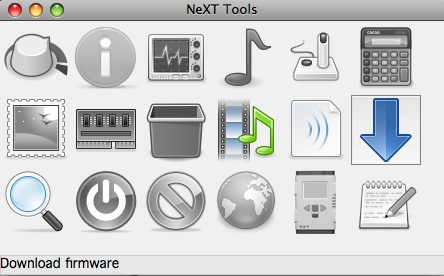
\includegraphics[width=0.7\textwidth]{pictures/firmware.jpg}
	\end{figure}
\item Remove the battery from the NXT and insert it again, and then press orange rectangle button on the NXT to turn on the Enhanced NXT firmware. The Enhanced NXT firmware has same GUI as the LEGO standard firmware.
\end{itemize}

%%%%
\subparagraph{Linux}
Note: Nextool binary for Linux seems to fail for firmware upload.\\
Install required packages:
\begin{verbatim}
$sudo apt-get install scons libusb-dev libusb-0.1-4
\end{verbatim}
Download the libnxt (\href{http://libnxt.googlecode.com/files/libnxt-0.3.tar.gz}{http://libnxt.googlecode.com/files/libnxt-0.3.tar.gz}) archive and extract it. Go in the new directory and build the project with scons:
\begin{verbatim}
$ cd libnxt-0.3/ 
$ scons
\end{verbatim}

A program call fwflash is created.\\
Download John Hansen's Enhanced NXT firmware (\href{http://bricxcc.sourceforge.net/lms_arm_jch.zip}{http://bricxcc.sourceforge.net/lms\_arm\_jch.zip}) (any version numbered 106 or later includes the native-invocation feature) and store the Enhanced NXT firmware (i.e lms\_arm\_nbcnxc\_1xx.rfw) in the directory where fwflash is stored.\\
Connect the NXT brick to usb and turn it on. Then press the reset button for more than 4s to put it in firmware upload mode (nxt display is cleared but it makes a ticking sound).\\
Flash the firmware with the following command (it takes some dozen of seconds), where 1xx is replaced by the number of the firmware:
\begin{verbatim}
$ sudo ./fwflash lms_arm_nbcnxc_1xx.rfw
\end{verbatim}

Troubleshooting: After completion of the upload, sometimes NXT display is messed and block : reboot it by a quick push on the reset button or remove the battery. If the NXT makes a ticking sound, it is still in firmware upload mode. If troubles, use and see windows firmware update procedure (and LEGO UserGuide).\\

%%%%
\subparagraph{Windows}
Download and install the Lego Drivers (\href{http://mindstorms.lego.com/en-us/support/files/default.aspx#Driver}{http://mindstorms.lego.com/en-us/support/files/default.aspx
\#Driver}) for PC. \\
Download Nexttool (\href{http://bricxcc.sourceforge.net/nexttool.zip}{http://bricxcc.sourceforge.net/nexttool.zip}) and a new firmware (\href{http://bricxcc.sourceforge.net/lms_arm_jch.zip}{http://bricxcc.sourceforge.net/lms\_arm\_jch.zip}) and update the firm-ware as explained below :
\begin{itemize}
\item Reset the NXT : To go into firmware update mode, press the reset button (at the back of the NXT, upper left corner beneath the USB connector) for more than 5 seconds while the NXT is turned on. The NXT will audibly tick when it is in firmware update mode.
\item Copy an Enhanced NXT firmware (i.e. lms\_arm\_nbcnxc\_107.rfw) to NeXTTool extracted directory.
\item Execute Cygwin and type the following command to change the current directory to the NexTTool extracted directory. (NeXTTool is assumed to be extracted under C:$\backslash$cygwin$\backslash$nexttool directory)
	\begin{verbatim}
	$cd C:\cygwin\nexttool
	\end{verbatim}
\item Connect PC and the NXT by USB cable.
\item Type the following command in Cygwin to upload the Enhanced NXT firmware to the NXT (Program upload may take around half minutes and then, NXT LCD is turned to display some chunk from blank).
	\begin{verbatim}
	$./NeXTTool.exe /COM=usb -firmware=lms\_arm\_nbcnxc\_107.rfw
	\end{verbatim}
\item Remove the battery from the NXT and insert it again, and then press orange rectangle button on the NXT to turn on the Enhanced NXT firmware. The Enhanced NXT firmware has same GUI as the LEGO standard firmware.
\end{itemize}




%%%%%%%%%%%%%%%%%%%%%%%%%
\paragraph{Upload a program}
\subparagraph{MAC OS}
To upload a program in the NXT (the nxt example examples/arm/nxt/simple/nxt\_simple\_exe.rxe)
\begin{itemize}
\item Connect the PC and the NXT by USB cable.
\item Launch Nexttool, select "usb port".
	\begin{figure}[htbp] %  figure placement: here, top, bottom, or page
   		\centering
		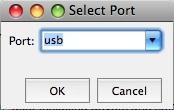
\includegraphics[width=0.25\textwidth]{pictures/usbport.jpg}
	\end{figure}
\item Go to "NXT Explorer"
	\begin{figure}[htbp] %  figure placement: here, top, bottom, or page
   		\centering
		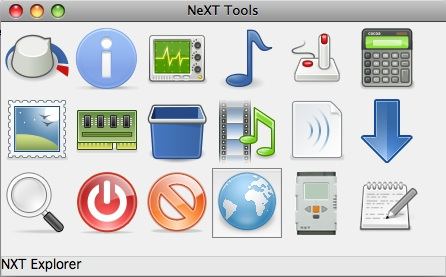
\includegraphics[width=.7\textwidth]{pictures/nxtexplorer.jpg}
	\end{figure}
\item Click on the "Download selected files to the NXT" and select the nxt\_simple\_exe.rxe file.
\item If program upload was succeeded, you can see the nxt\_simple\_exe.rxe file in the files list as below.
	\begin{center}[h] %  figure placement: here, top, bottom, or page
   		%\centering
		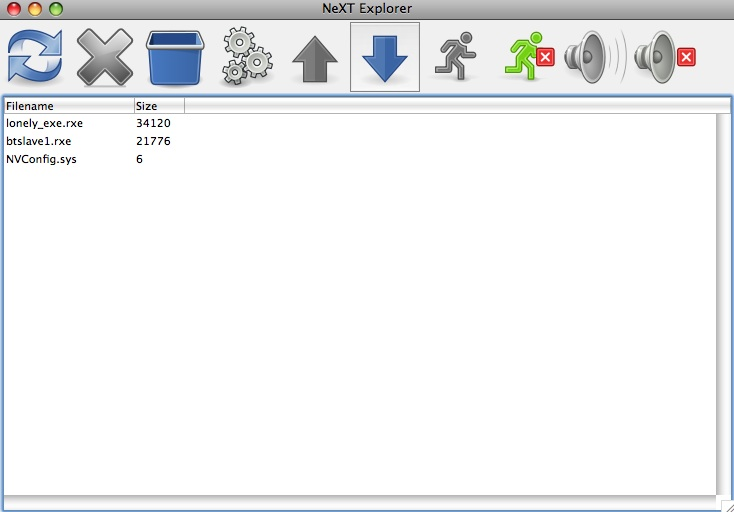
\includegraphics[width=1\textwidth]{pictures/downloadfile.jpg}
	\end{center}
\item To execute a program on the NXT, go in "My files"/"Software files".
\end{itemize}

%%%%
\subparagraph{Linux}
Required Packages: libusb-0.1-4\\
Download this executable of John Hansen's NeXTTool (\href{http://lejos-osek.sourceforge.net/installation_linux_files/NeXTTool}{here}) (built from bricxcc svn repository, revision 1)\\
Check the version of NeXTTool, it should be 1.0.1.0:
\begin{verbatim}
$ sudo ./[NEXTTOOL_PATH]/NeXTTool
nexttool version 1.0.1.0 (1.0.1.0)
Copyright (c) 2006, John Hansen
Use "NeXTTool -help" for more information.
\end{verbatim}

To ubload over usb, turn on the NXT, connect it to USB and run the following command (example: nxt\_simple\_exe.rxe) :
\begin{verbatim}
$ sudo ./[NEXTTOOL_PATH]/NeXTTool /COM=usb -download=nxt\_simple\_exe.rxe
\end{verbatim}

Troubleshooting: Test the following command to see if Nexttool is working (set execution right for NeXTTool):
\begin{verbatim}
$ sudo ./[NEXTTOOL_PATH]/NeXTTool /COM=usb -versions
Protocol version = 1.124
Firmware version = 1.xx
\end{verbatim}

To ubload over bluetooth, you need to define an alias name in a file 'nxt.dat' as explained in this post: Minsdtorm 2.0 development on linux . Then turn on the NXT and run the following command (example: nxt\_simple\_exe.rxe) :
\begin{verbatim}
$ sudo ./[NEXTTOOL_PATH]/NeXTTool /COM=alias_bt -download=nxt\_simple\_exe.rxe
\end{verbatim}

To execute a program on the NXT, go in "My files"/"Software files".

%%%%
\subparagraph{Windows}
To upload a program in the NXT (the nxt example examples/arm/nxt/lonely\_exe.rxe) follow the steps below :
\begin{itemize}
\item Connect the PC and the NXT by USB cable.
\item Type the following command in Cygwin (from examples/arm/nxt) :
	\begin{verbatim}
	$./[NEXTTOOL_PATH]/NeXTTool.exe /COM=usb -download=lonely_exe.rxe
	$./[NEXTTOOL_PATH]/NeXTTool.exe /COM=usb -listfiles=lonely_exe.rxe
	\end{verbatim}
\item If program upload was succeeded, program size could be displayed in Cygwin such as the second line in the below command outputs. 
	\begin{verbatim}
	Executing NeXTTool to upload helloworld.rxe...
	helloworld.rxe=15280
	NeXTTool is terminated.
	\end{verbatim}
\item To execute a program on the NXT, go in "My files"/"Software files".
\end{itemize}


\subsubsection{Olimex LPC-E2294}

%%%%%%%%%%%%%%%%%%%%%%%%%
\paragraph{OPENOCD + drivers}
%%%%%%
openOCD is a software that communicates via the JTAG (Open On-Chip Debug Solution for Embedded Target Systems based on the ARM7 and ARM9 Family). It's an open source software by BerliOS (http://openocd.berlios.de/web/). \\
Download and compile openOCD for your achitecture (it appears revision after 1200 are not able to compile correcty under MacOS X).\\
As you don't need just openOCD because it needs the USB driver, you've got two choice : 
\begin{itemize}
\item install libusb et libftdi
\item install D2XX
\end{itemize}

%%%%%%%%%%%%%%%%%%%%%%%%%
\paragraph{Upload a program}
To upload a program double click on \textit{2-run-openocd.command} to open the connection between your computer and the board.\\
And double click on \textit{2a-debug-external-ram.command} if you want to upload your program in external ram with debug.\\
In the debug consol type :
\begin{itemize}
\item "c" to continue
\item "b" to place a breakpoint
\item "si" to step instruction
\item "display/i \$pc" to display assembler code on the pc register
\item "x/i \$pc" to visualise the i blocs from pc
\item "info registers" to see the registers state
\end{itemize}








%\newpage
\chapter{Appendix}
%%%%%%%%%%%%%%%%%%%%%%%%%
\section{Launching Trampoline tests} \label{tests}
To launch the tests you have to compile ViPER \footnote{Virtual Processor Emulator, ViPER is used on Posix system to send interrupts to Trampoline to emulate the timers. It is launched by Trampoline.} first. Go in viper/ and type in a terminal :
	\begin{verbatim}
	$make
	\end{verbatim}
To launch the tests, go in check/ and type in a terminal :
	\begin{verbatim}
	$./tests.sh
	\end{verbatim}
At the end of the tests you should see :
	\begin{verbatim}
	...
	Compare results with the expected ones...
	Functional tests Succeed!!
	GOIL tests Succeed!!
	\end{verbatim}
If an error occurs, you can visit Trampoline's forum (\href{http://trampoline.rts-software.org/bb/}{http://trampoline.rts-software.org/bb/}).


%%%%%%%%%%%%%%%%%%%%%%%%%
\section{Cross-Compile an application} \label{compileanapplication}
To cross-compile a Trampoline application for ARM for example, you need to set  :
\begin{verbatim}
COMPILER = "arm-elf-gcc";
ASSEMBLER = "arm-elf-as";
LINKER = "arm-elf-ld";
\end{verbatim}
in your oil file as you can see in examples/arm/nxt/nxt\_simple.oil.\\
For the Lego Mindstorm NXT2.0 only, you also need to add the path to your libgcc and libc as below (X.X.X is your cross-gcc version) :
\begin{verbatim}
LDFLAGS = "-L[GNUARM_PATH]/lib/gcc/arm-elf/X.X.X -lgcc";
LDFLAGS = "-L[GNUARM_PATH]/arm-elf/lib -lc";
\end{verbatim}

And then, compile your application typing in a terminal (from the example in examples/arm/nxt/simple) :
	\begin{verbatim}
	$goil -t=arm/nxt --templates=../../../../goil/templates -g -i nxt_simple.oil
	\end{verbatim}
This will generate the Makefile needed, thus type :
	\begin{verbatim}
	$make
	\end{verbatim}
Then you need to upload the nxt\_simple\_exe.rxe file after installing drivers and softwares on your platform.



\printindex
\end{document}  